\documentclass[a4paper,12pt]{report}

\usepackage{alltt, fancyvrb, url}
\usepackage{graphicx}
\usepackage[utf8]{inputenc}
\usepackage{float}
\usepackage{hyperref}

\usepackage[italian]{babel}

\usepackage[italian]{cleveref}

\title{''Ralph Spaccatutto''}

\author{Enrico Cornacchia \\ Giulia Golesano \\ Giovanni Rinchiuso \\ Nikolai Zanni}
\date{10 giugno 2024}

\begin{document}

\maketitle

\tableofcontents

\chapter{Analisi}

\section{Requisiti}

Il progetto si pone l'obbiettivo di ricreare un videogioco basato sul film Ralph Spaccatutto, che rientra nella categoria dei giochi platformer, ossia dei giochi in cui la meccanica di gioco implica l'attraversamento di uno o piu livelli, ognuno dei quali è composto da piattaforme solitamente situate su più piani.

\subsection{Requisiti funzionali}

\begin{itemize}

	\item Felix, il protagonista del gioco, avrà l'obiettivo di aggiustare tutte le finestre del condominio, rotte dall'antagonista Ralph. 
	\item Per arrivare a tale scopo, potrà muoversi a destra e a sinistra lungo ogni piattaforma, che rappresenta un piano del condominio, per poi salire o scendere agli altri piani.
	\item Una complicazione che incontrerà il protagonista sono i mattoni che, durante tutta la partita, Ralph lancerà dalla sua piattaforma in cima al condominio.
 \item Felix  dovrà schivare i mattoni per non perdere le sue 3 vite a disposizione.
	\item Degli aiuti che potrà ottenere sono invece i power ups.
	\item I nostri requisiti funzionali prevedono, oltre al corretto funziamento del gioco, una schermata iniziale da cui selezionare il livello e l'avvio e un menù di pausa per arrestare il gioco, tramite appositi tasti.
\end{itemize}

\subsubsection{Requisiti non funzionali}
\begin{itemize}
	\item Ci poniamo l'obiettivo di fornire un'esperienza di gioco il più fluida possibile, restando sempre fedeli alla versione originale nonostante le nostre rivisitazioni.
\end{itemize}

\section{Analisi e modelli del dominio}
La schermata di gioco è composta da una facciata di condominio, simile ad una griglia, in cui si trovano alcune file di finestre, alcune intere e alcune rotte, in base alla difficoltà del livello.
Come anticipatamente spiegato, il player Felix dovrà aggiustare tutte le finestre, schivando i mattoni lanciati da Ralph, per vincere la partita.
Per farlo, dovrà fermarsi, davanti alla finestra che desidera aggiustare, e tenere premuto il tasto Z per 1.5 secondi. 
Per muoversi tra i piani avrà a disposizione le 4 direzioni UP, DOWN, LEFT e RIGHT, ognuna svolta dalle lettere W,S,A e D.
Felix avrà un numero limitato di vite, che di default sarà 3, che potrà perdere se colpito da uno dei mattoni lanciati da Ralph.
Durante il gioco saranno possibili power ups che permetteranno a Felix di ricevere aiuti extra.
Ci sono due tipi di power-ups: le torte che garantiscono a Felix invincibilità per dieci secondi e gli uccelli che bloccano Ralph dal lanciare mattoni sempre per dieci secondi.
Con l'aumentare del livello, Ralph lancia più mattoni, i mattoni cadono più velocemente, compaiono meno power-ups e ci sono più finestre da aggiustare nella schermata di partenza. 


\begin{figure}[H]
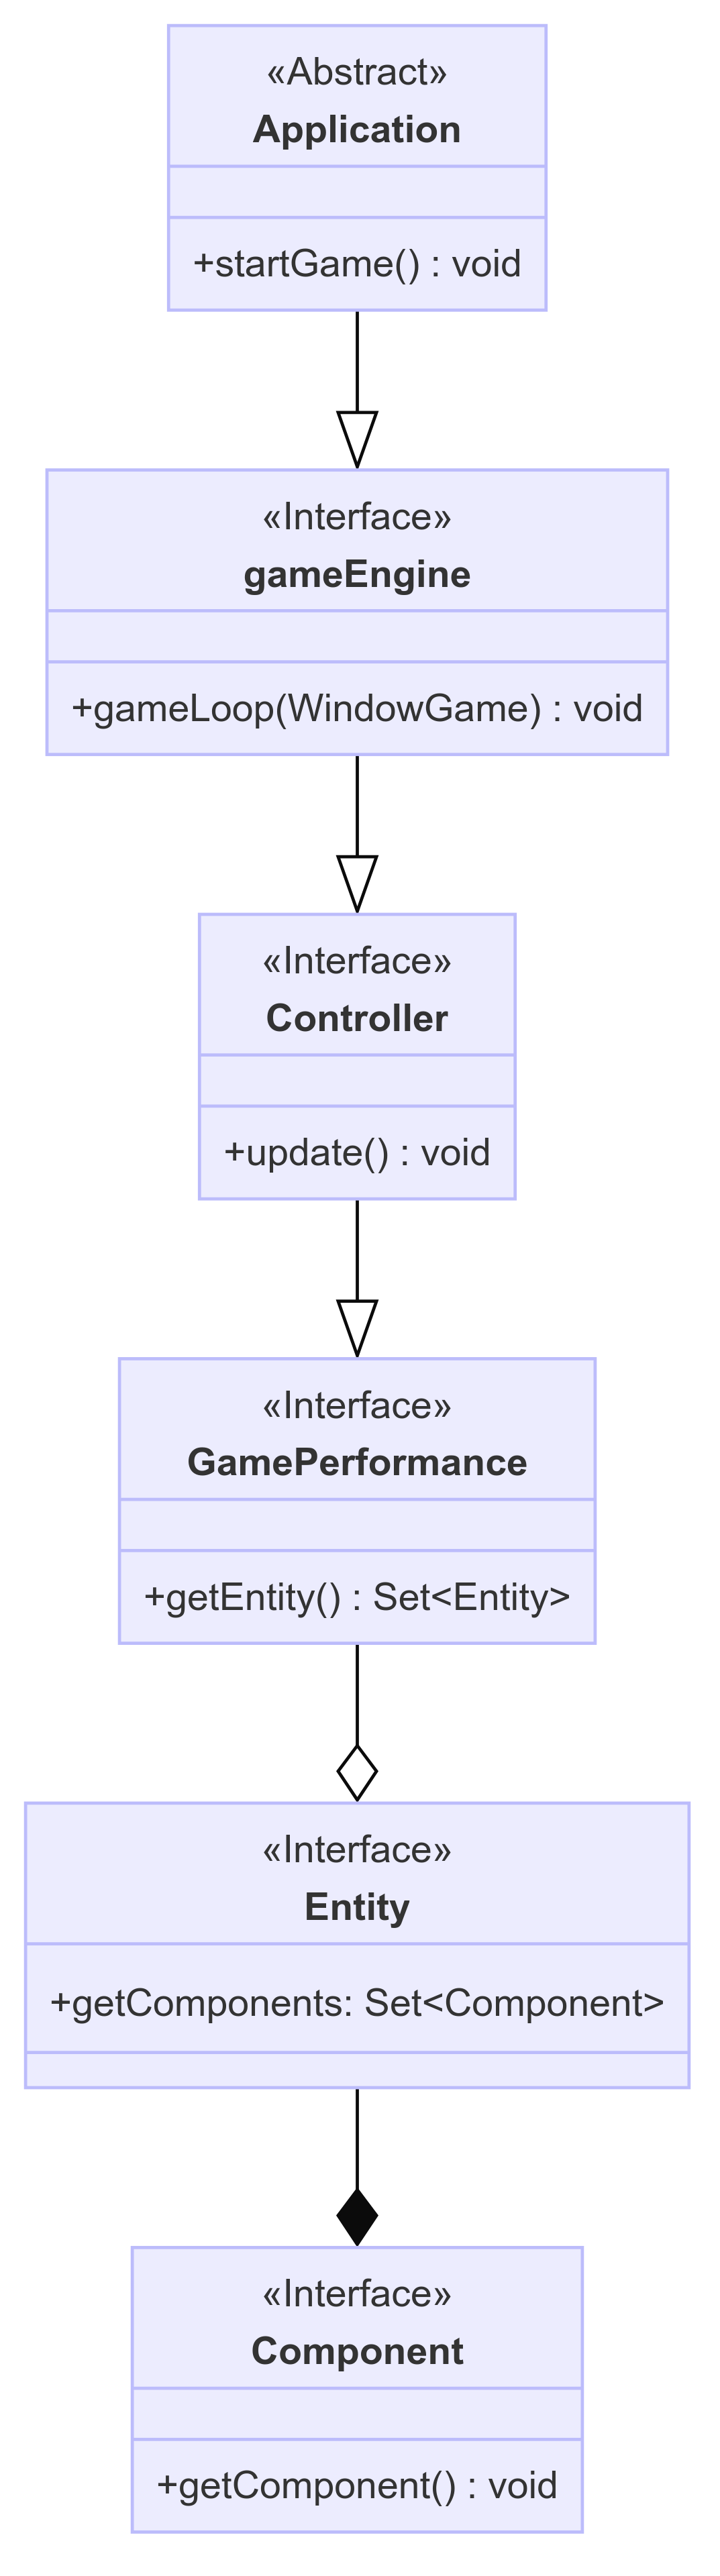
\includegraphics[width=0.4\textwidth]{img/analisi.png} 
\centering{}
\caption{Schema UML dell'analisi del problema, con rappresentate le entità principali ed i rapporti fra loro}
\label{img:analisi}
\end{figure}

\chapter{Design}

\section{Architettura}
Per realizzare il progetto abbiamo adottato il pattern architetturale MVC (Model-View-Controller) rispettando il più possibile tale suddivisione. 
Ogni suddivisione gestisce una parte diversa: "model” gestisce la logica e i dati del gioco, “view” gestisce la parte grafica, che in base allo stato di gioco (menu, playing, settings, win, gameover, paused) disegnerà la corretta schermata, infine “controller” ha il compito di interporsi tra model e view per permetterne la comunicazione. 
Abbiamo inoltre scelto di adottare il pattern ECS (Entity-Component System) per la parte di Model, in particolare ogni oggetto di gioco é un’entità che può essere composta da componenti, ognuno dei quali descrive uno specifico comportamento. 

\begin{figure}[H]
\centering{}
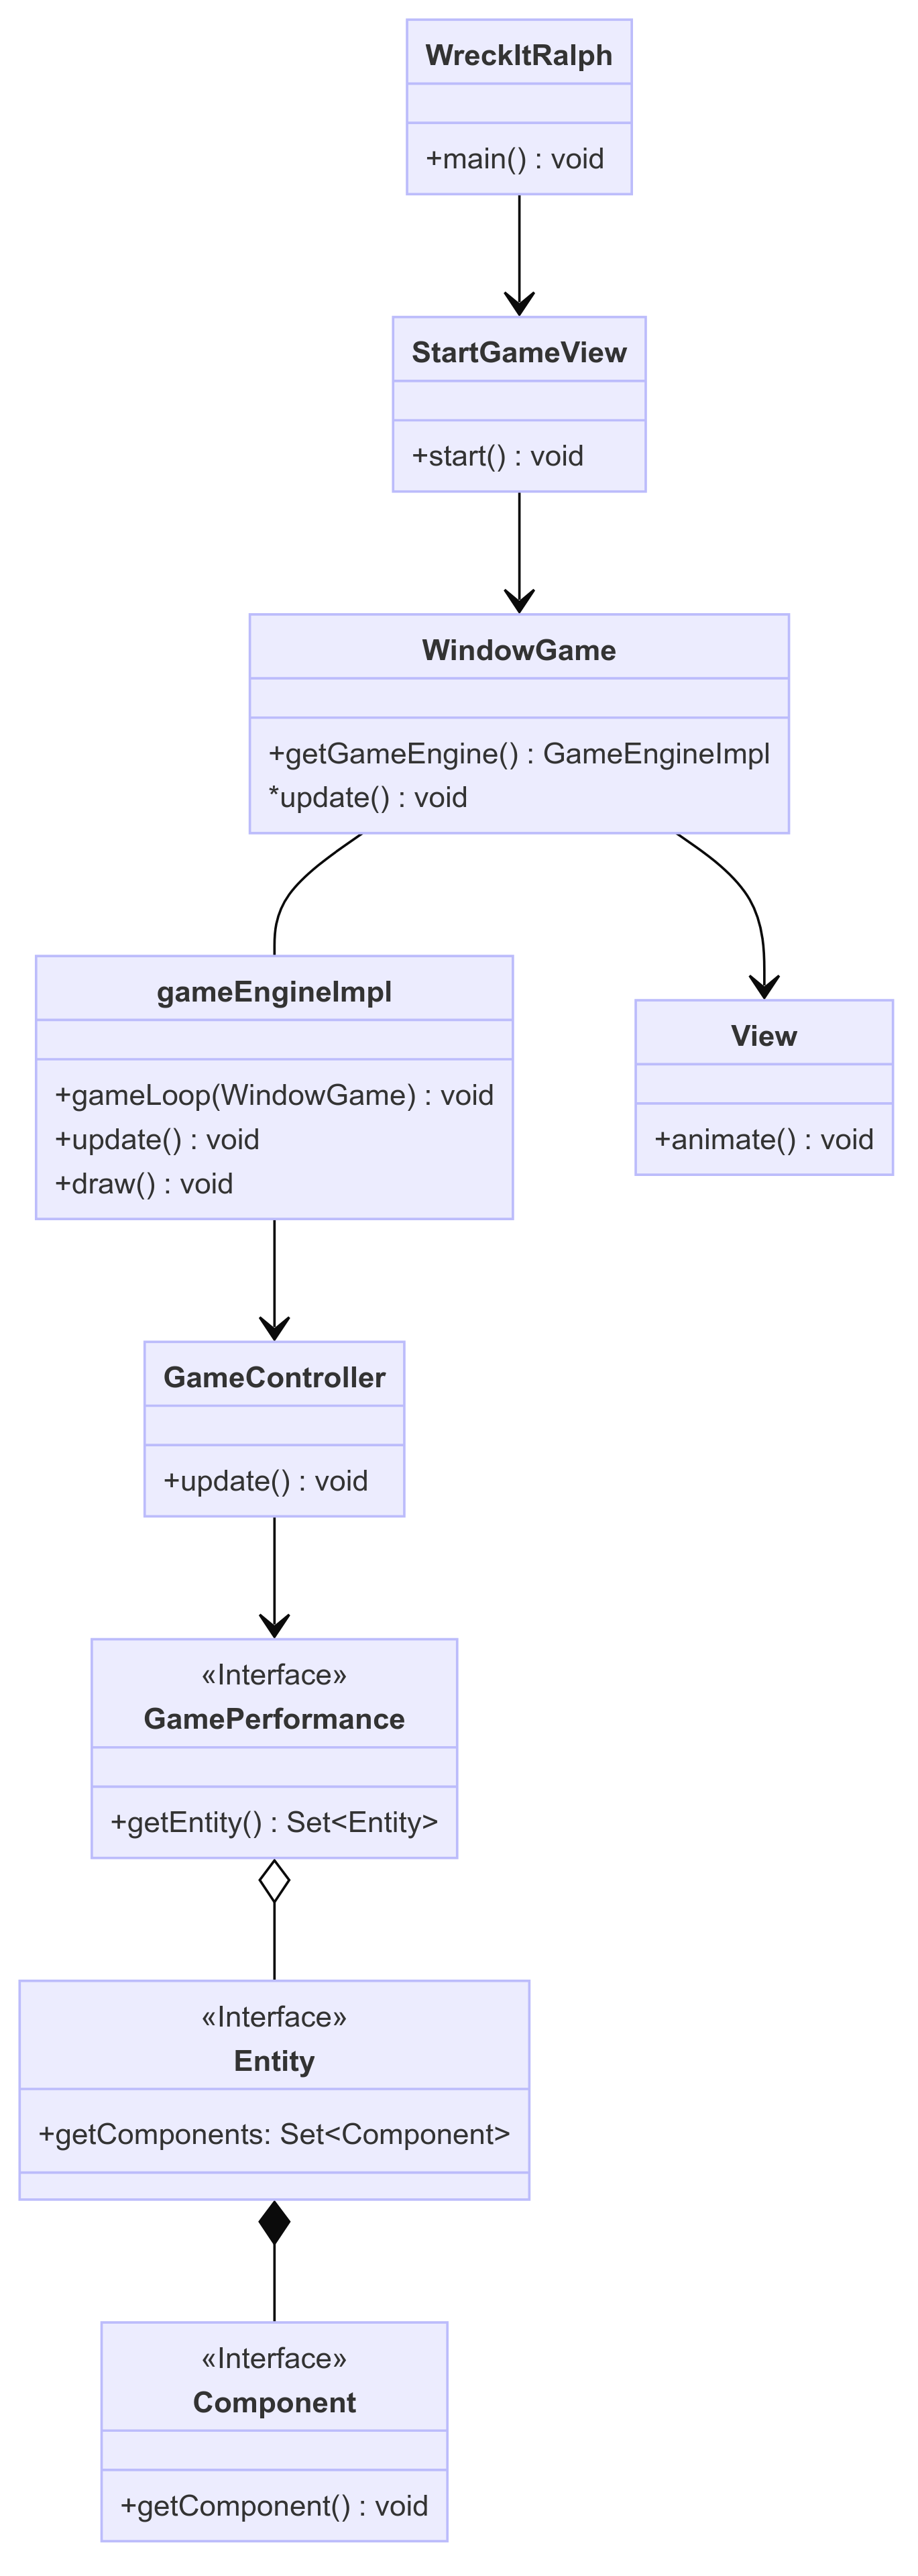
\includegraphics[width=0.4\textwidth]{img/architettura.png}
\caption{Schema UML architetturale di DonkeyKong.}
\label{img:architettura}
\end{figure}

\section{Design dettagliato}
\subsection{Nikolai Zanni}

\subsubsection{Implementazione del menù.}

\begin{figure}[H]
\centering{}
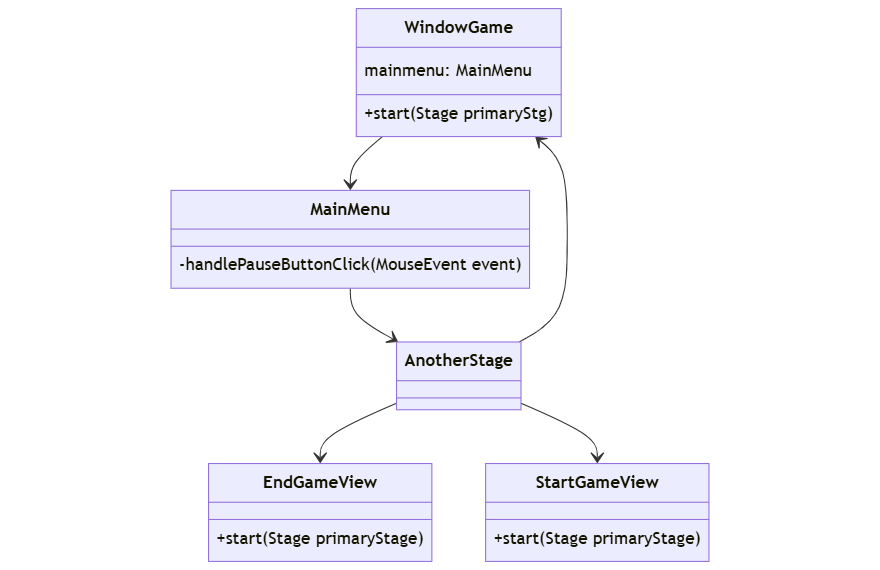
\includegraphics[width=0.9\textwidth]{img/mainmenu.png}
\caption{Rappresentazione UML della gestione del menù.}
\end{figure}

\paragraph{Problema:}
Duarnte il corso della partita è possibile usare il menù per mettere il gioco in pausa. 
Dal menu è possibile poter tornare a riprendere la partita, oppure andare alla schermata inziale o quella finale.

\paragraph{Soluzione:}
Per implementare il menù del gioco, ho creato la classe MainMenu, che utilizza JavaFX per gestire l'interfaccia grafica e offre una serie di funzionalità che permettono all'utente di controllare lo stato del gioco. 
La classe MainMenu è responsabile della creazione e gestione di un pulsante di pausa che, cliccato, mette in pausa il gioco e apre una nuova finestra rappresentata dalla classe interna AnotherStage, che estende Stage. 
La classe AnotherStage è progettata per gestire la finestra del menù di pausa. 
Include tre pulsanti: "resume" , "quit" e "home". 
Questi pulsanti permettono rispettivamente di riprendere il gioco, chiudere il gioco e tornare alla schermata principale. 

\subsubsection{Implementazione e gestione delle entità dei power-ups}

\begin{figure}[H]
\centering{}
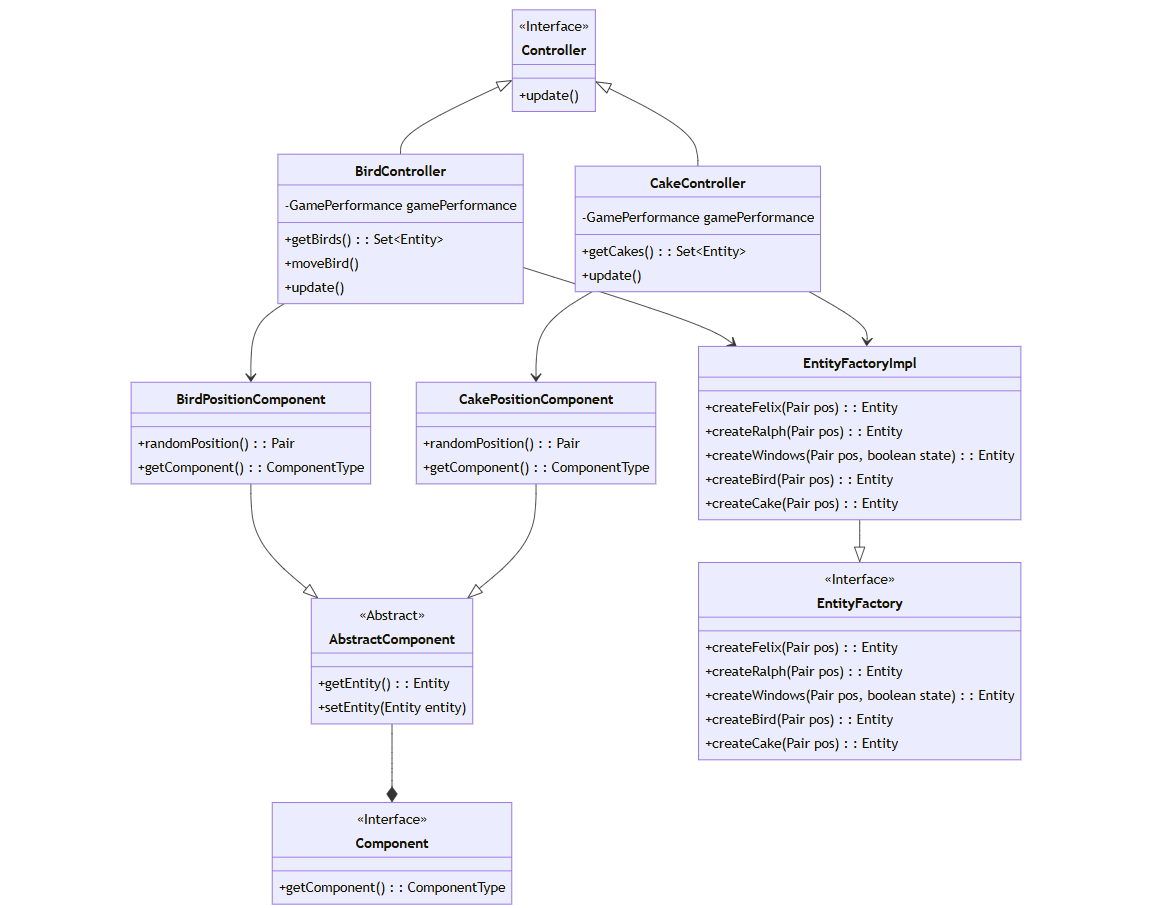
\includegraphics[width=0.9\textwidth]{img/powerups.png}
\caption{Rappresentazione UML della gestione dei power-ups.}
\end{figure}

\paragraph{Problema:}
All'interno del gioco abbiamo delle entità che rappresentano i power-ups. 
L'entià Bird dovrà bloccare Ralph dalla possibilità di lanciare i mattoni, mentre l'entità Cake invece dovrà rendere Felix invincibile. 
Queste due entità saranno presenti nel gioco ad intervallo di tempo che dipenderà dalla scelta inziale della difficoltà. 

\paragraph{Soluzione:}
Per l'implementazione dei power-up Bird e Cake, ho deciso di utilizzare il Factory Pattern nella classe EntityFactoryImpl e di creare componenti specifici per ognuno di essi. 
Il componente BirdPositionComponent posiziona i birds in modo casuale su uno dei tre piani del gioco, mentre il componente CakePositionComponent posiziona i cakes su finestre scelte casualmente. 
Tramite il BirdController gestisco la creazione e il movimento dei birds, mentre tramite il CakeController gestisco la creazione e la durata attiva dei cakes.

\subsubsection{Gestione dell'abilità del power-up Cake e gestione vite.}

\begin{figure}[H]
\centering{}
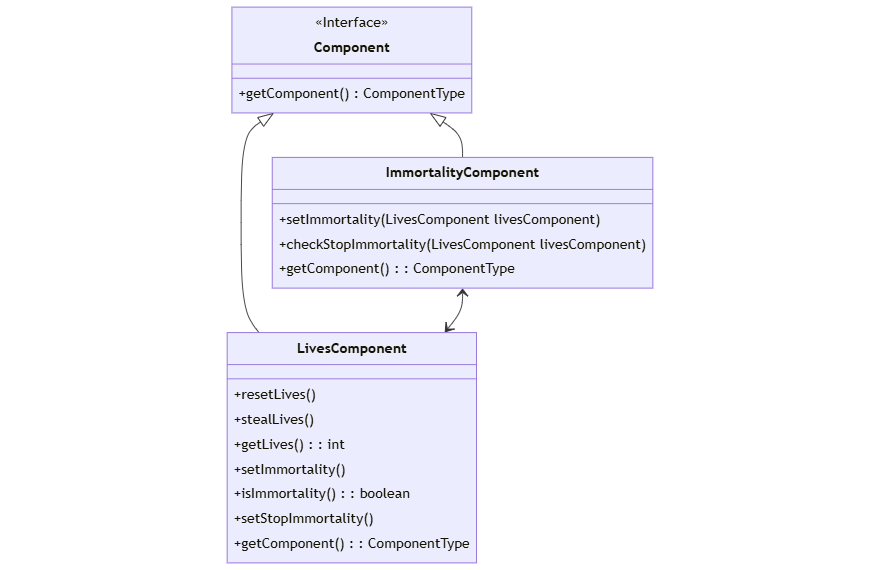
\includegraphics[width=0.9\textwidth]{img/immortalityelife.png}
\caption{Rappresentazione UML della gestione dell'abilità di Cake e gestione delle vite}
\end{figure}

\paragraph{Problema:}
Il mio power-up Cake nel gioco, se preso, deve poter rendere invincibile l'entità che entra in contatto con Cake. 
L'invincibilità deve durare per un periodo di tempo definito, durante il quale l'entità non può perdere vite.

\paragraph{Soluzione:}
Per la gestione dell'abilità di Cake, ho deciso di implementare un componente chiamato ImmortalityComponent che si occupa di gestire lo stato di immortalità dell'entità che entra in contatto con il power-up. 
Questo componente interagisce con il LivesComponent, che gestisce le vite dell'entità. 
Quando un'entità raccoglie un Cake, il LivesComponent abilita l'immortalità, prevenendo la perdita di vite per un periodo di tempo definito. 
Il contatto tra l'entità e il power-up Cake viene verificato tramite il componente HitboxComponent, che gestisce le collisioni tra le entità nel gioco. 
Quando viene rilevata una collisione tra l'entità e un Cake, il ImmortalityComponent viene attivato per abilitare l'immortalità nel LivesComponent. 
L'Observer Pattern è implementato nel LivesComponent per notificare i cambiamenti nelle vite dell'entità ai listener registrati. 

\subsubsection{Gestione dei punti.}

\begin{figure}[H]
\centering{}
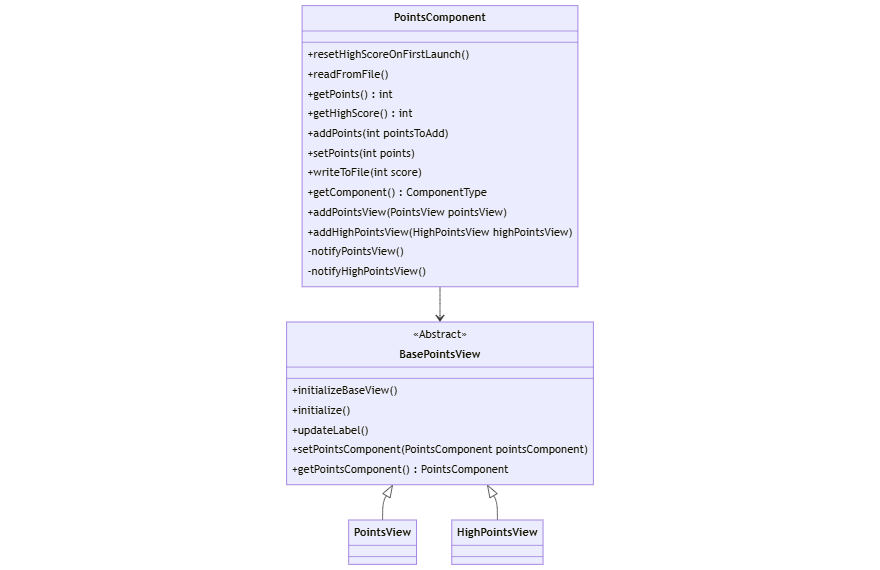
\includegraphics[width=0.9\textwidth]{img/points.png}
\caption{Rappresentazione UML della gestione dei punti.}
\end{figure}

\paragraph{Problema:}
Nel gioco, è necessario gestire i punti accumulati quando si aggiusta una finestra. 
Inoltre, è importante mantenere traccia del punteggio più alto raggiunto e visualizzare queste informazioni nell'interfaccia utente. 
I punti devono essere aggiornati in tempo reale e salvati tra una sessione di gioco e l'altra. 
Il punteggio maggioere deve anche poter essere resettato ogni volta che si apre il gioco.

\paragraph{Soluzione:}
Per risolvere questo problema, ho implementato un componente chiamato PointsComponent che si occupa di gestire i punti accumulati da un'entità e il punteggio più alto raggiunto. 
Questo componente è responsabile della lettura e scrittura dei punteggi su un file per preservare le informazioni tra le sessioni di gioco. 
Inoltre, utilizza il pattern Observer per aggiornare le viste dei punti e del punteggio più alto ogni volta che questi cambiano. 
Quando il gioco inizia, il componente legge il punteggio più alto da un file. 
Inoltre, notifica le viste dei punti (PointsView e HighPointsView) di aggiornare le loro etichette per riflettere i nuovi valori. 
La gestione della persistenza dei dati è realizzata utilizzando lettura e scrittura su file tramite BufferedWriter e BufferedReader. 
L'Observer Pattern è implementato nel PointsComponent per notificare le viste (PointsView e HighPointsView) quando i punti o il punteggio più alto cambiano. 


\subsection{Cornacchia Enrico}

\subsubsection{Gestione di entità}

\begin{figure}[H]
\centering{}
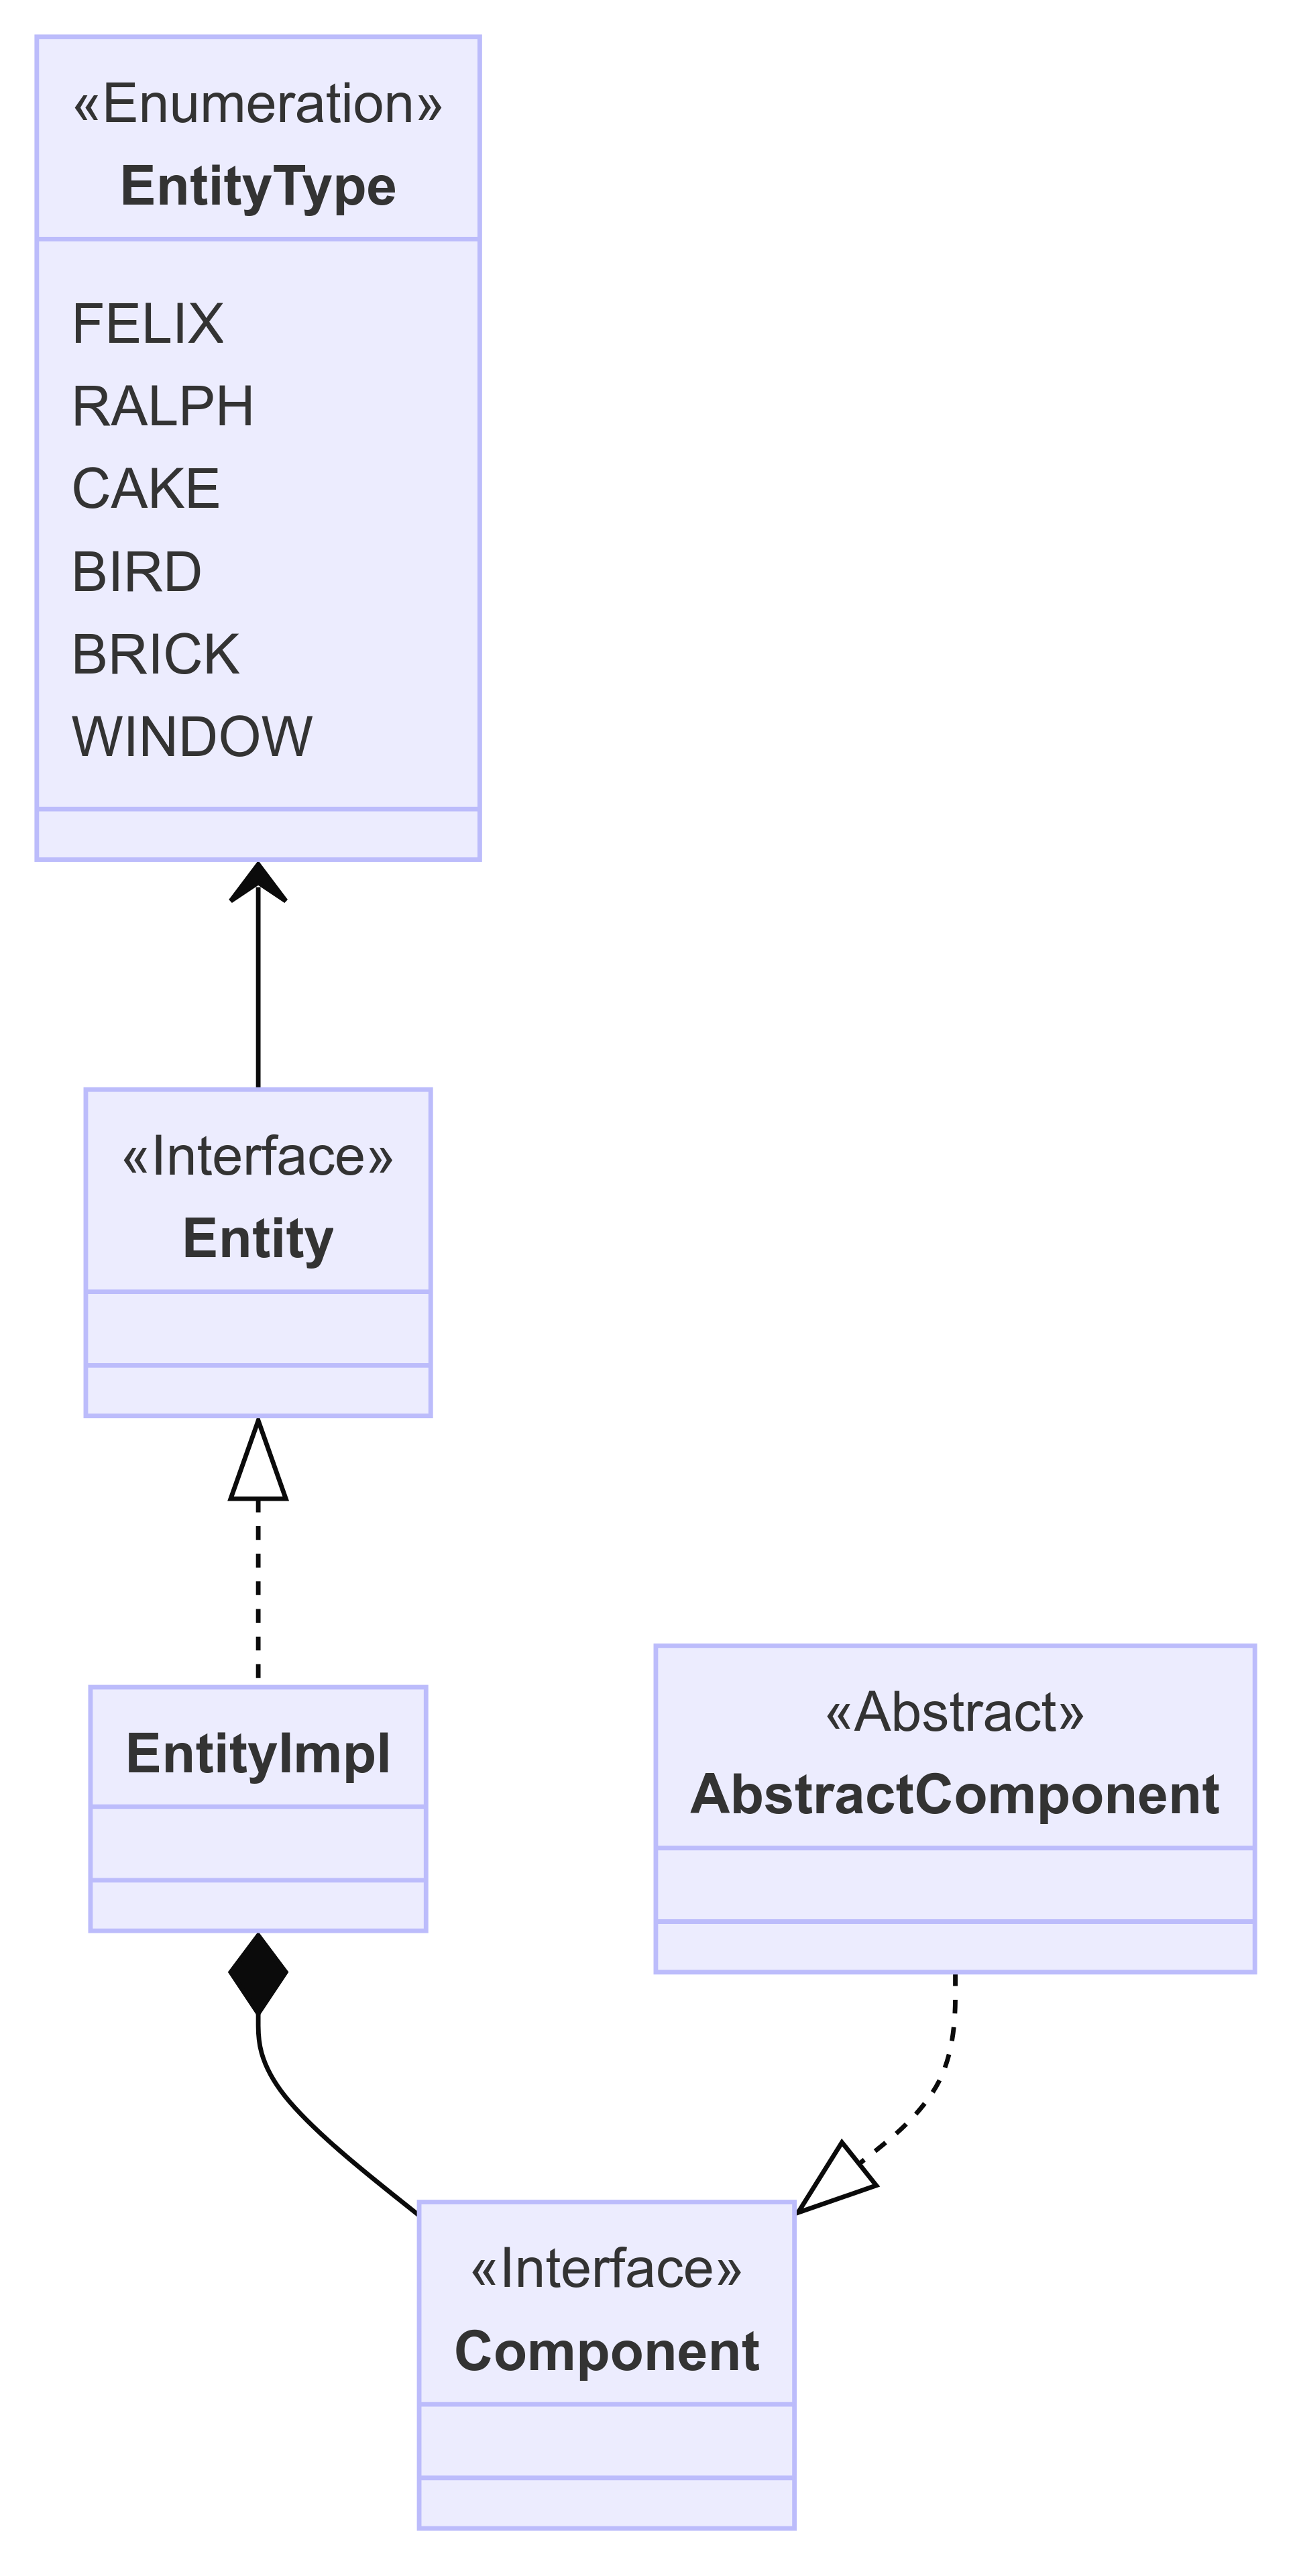
\includegraphics[width=0.4\textwidth]{img/entities.png}
\caption{Rappresentazione UML dell'implementazione delle entità.}
\end{figure}

\paragraph{Problema:}
Nel contesto di un gioco, le entità sono elementi centrali e la loro gestione deve essere efficiente. In particolare, è comune che diverse entità condividano comportamenti simili o identici, il che può portare a duplicazione di codice. 

\paragraph{Soluzione:}
Per affrontare il problema della duplicazione di codice e gestire in modo efficiente le entità, ho adottato il Composite pattern. In questo approccio, ogni entità è rappresentata da una singola classe, con enumeratore che ne identifica la tipologia. Questa classe può essere vista come un contenitore vuoto che può essere arricchito con vari componenti durante la sua creazione. Questi componenti, che rappresentano comportamenti o caratteristiche specifiche, possono essere combinati in vari modi per creare entità diverse. Questo rende il codice più modulare, facilita le modifiche e le estensioni, e promuove il riutilizzo del codice. 

\subsubsection{Creazione di nuove entità}

\begin{figure}[H]
\centering{}
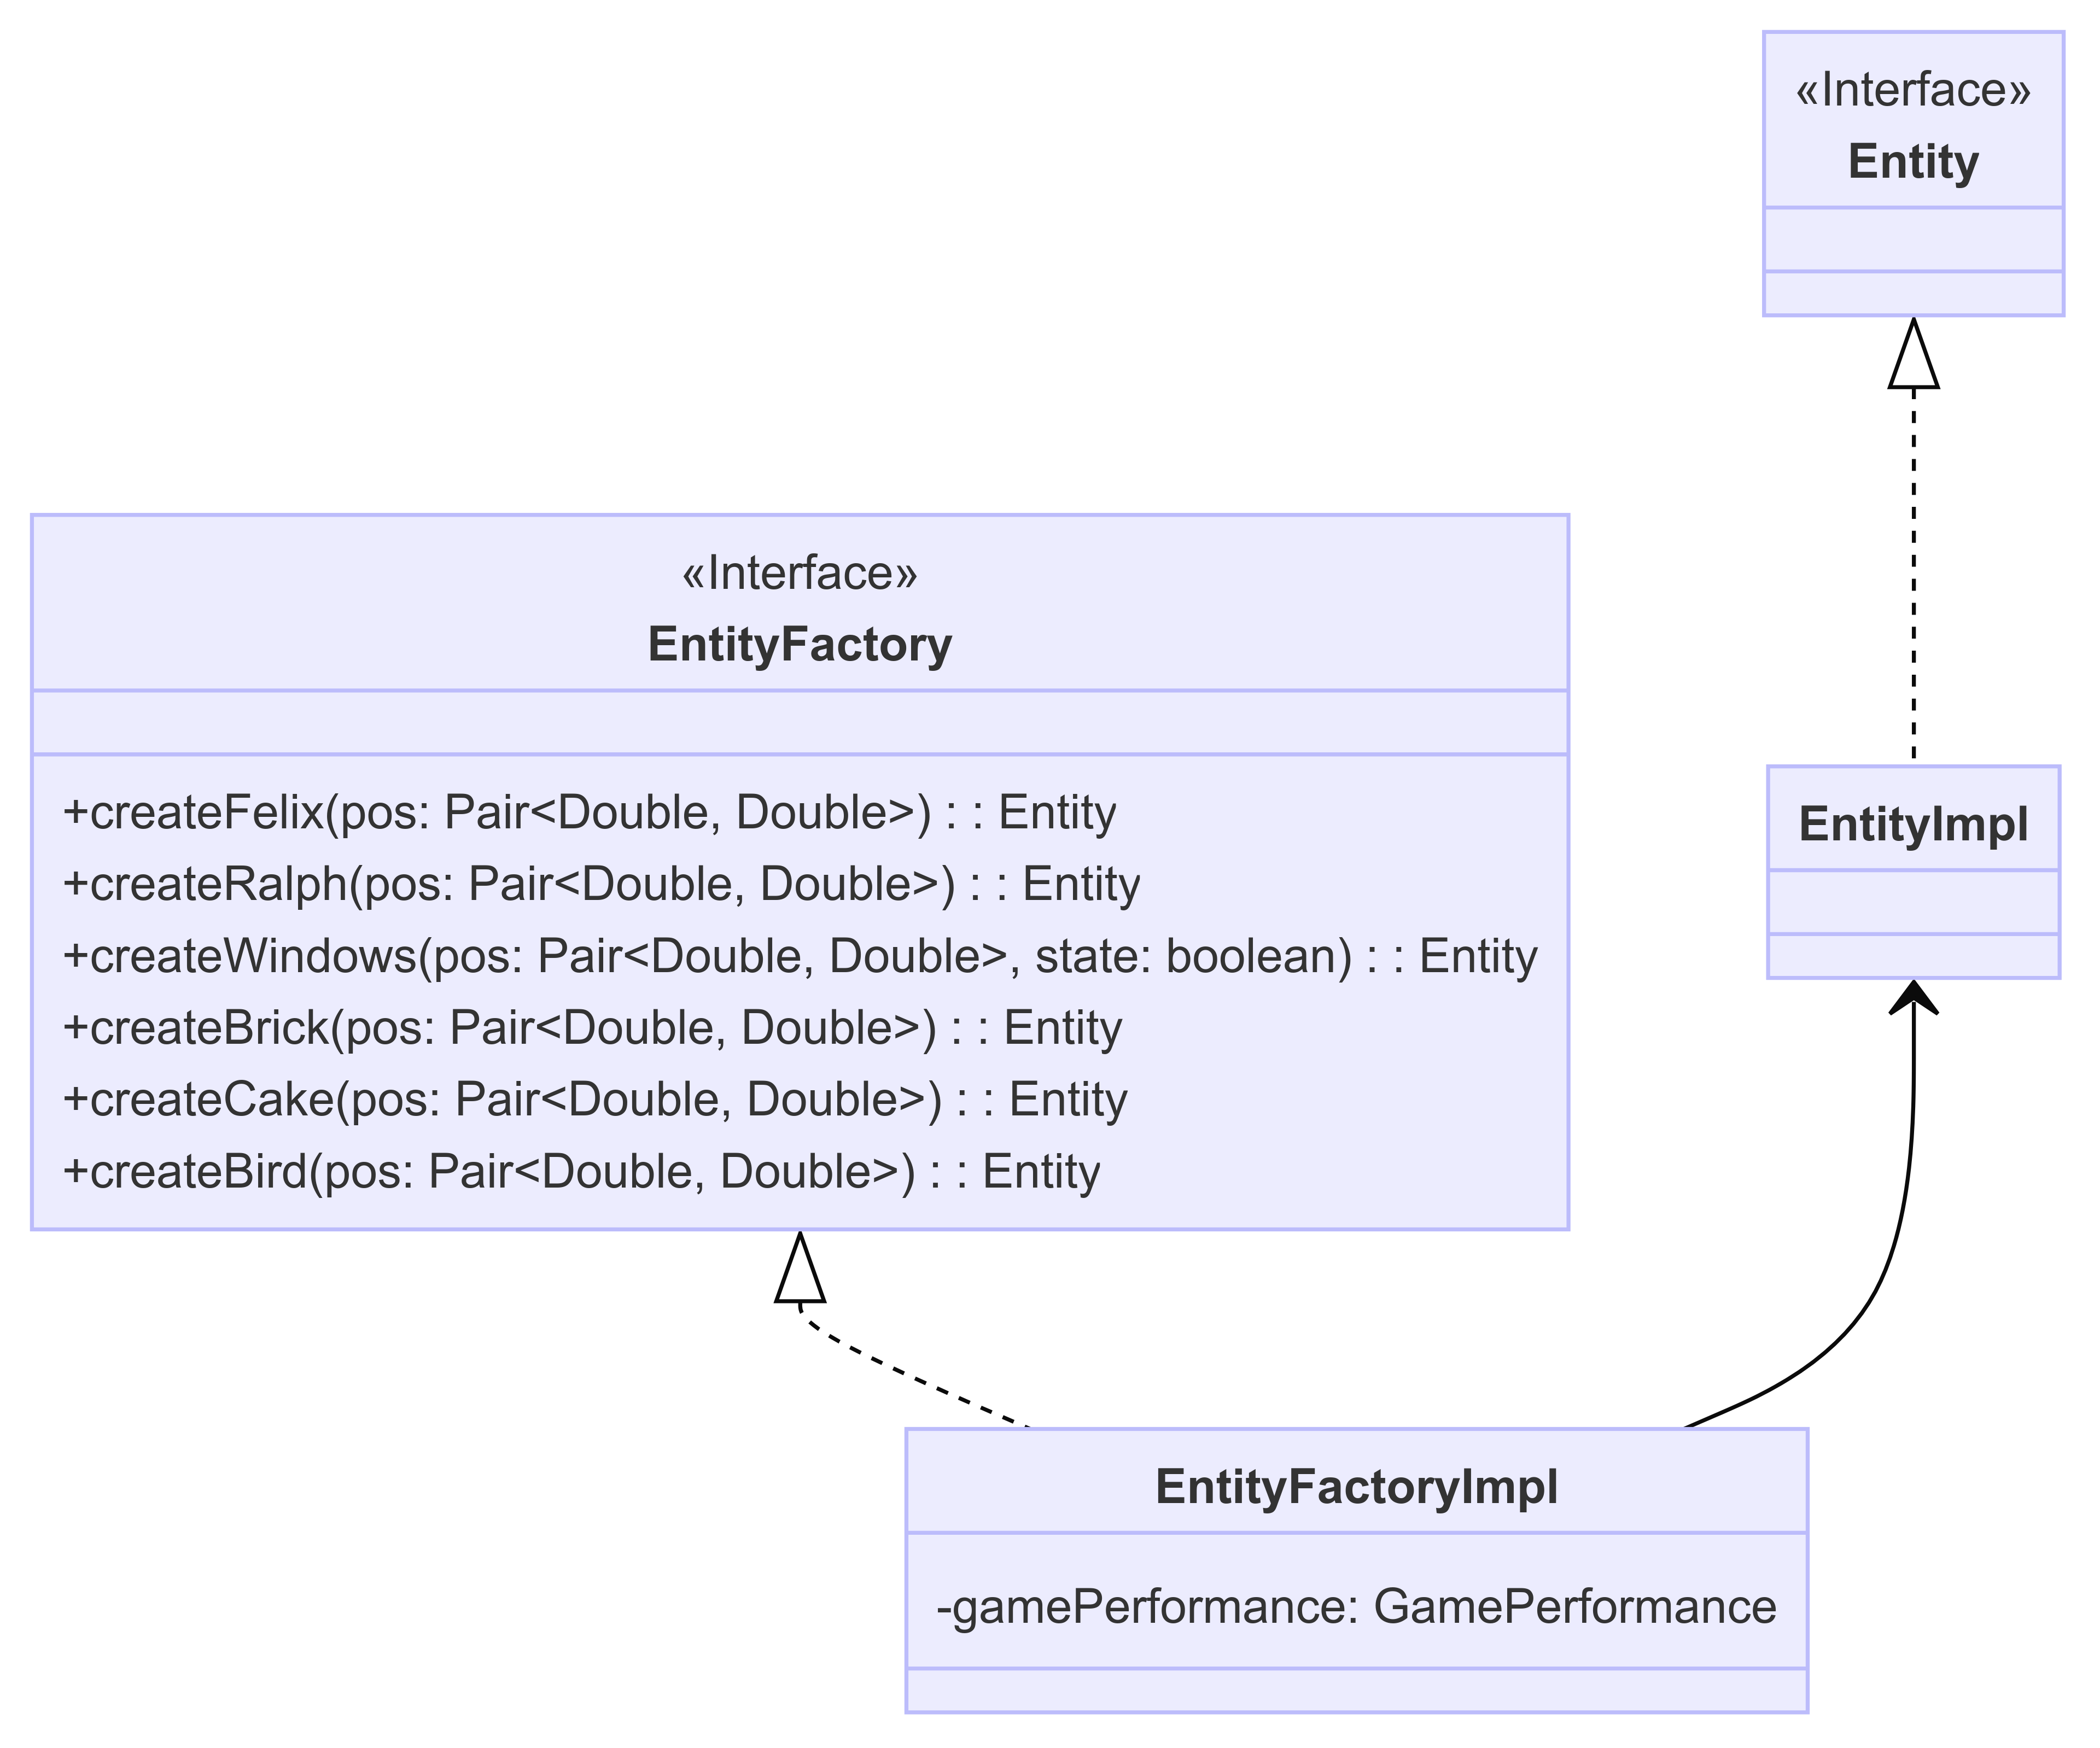
\includegraphics[width=0.9\textwidth]{img/entity_factory.png}
\caption{Rappresentazione UML della creazione di entità.}
\end{figure}

\paragraph{Problema:}
Sia in fase di avvio del gioco che nel corso dello stesso, è indispensabile generare varie entità, ciascuna con diversi componenti, a seconda dei comportamenti definiti per ciascuna.

\paragraph{Soluzione:}
Ho, quindi, usato il Factory pattern visto che permette di generare nuove istanze di entità in maniera centralizzata, ognuna diversa e con componenti vari, in modo relativamente veloce e semplice. Ciò comporta numerosi benefici, tra cui la separazione della logica di creazione delle entità dal resto dell'applicazione, rendendo il codice più modulare. Inoltre, in futuro, se fosse necessario modificare la creazione, i parametri o i componenti di una o più entità, ciò potrebbe essere fatto con maggiore facilità. La factory può accettare parametri in ingresso per la creazione di queste entità, come ad esempio la posizione o lo stato iniziale. In alternativa si sarebbe potuto usare anche il Builder Pattern, tuttavia le entità in questo gioco non richiedono particolari passaggi per la loro creazione e avere classi builder per ogni tipo di entità renderebbe complesso il codice più di quanto sia necessario in questo caso.

\subsubsection{Gestione delle collisioni tra entità}

\begin{figure}[H]
\centering{}
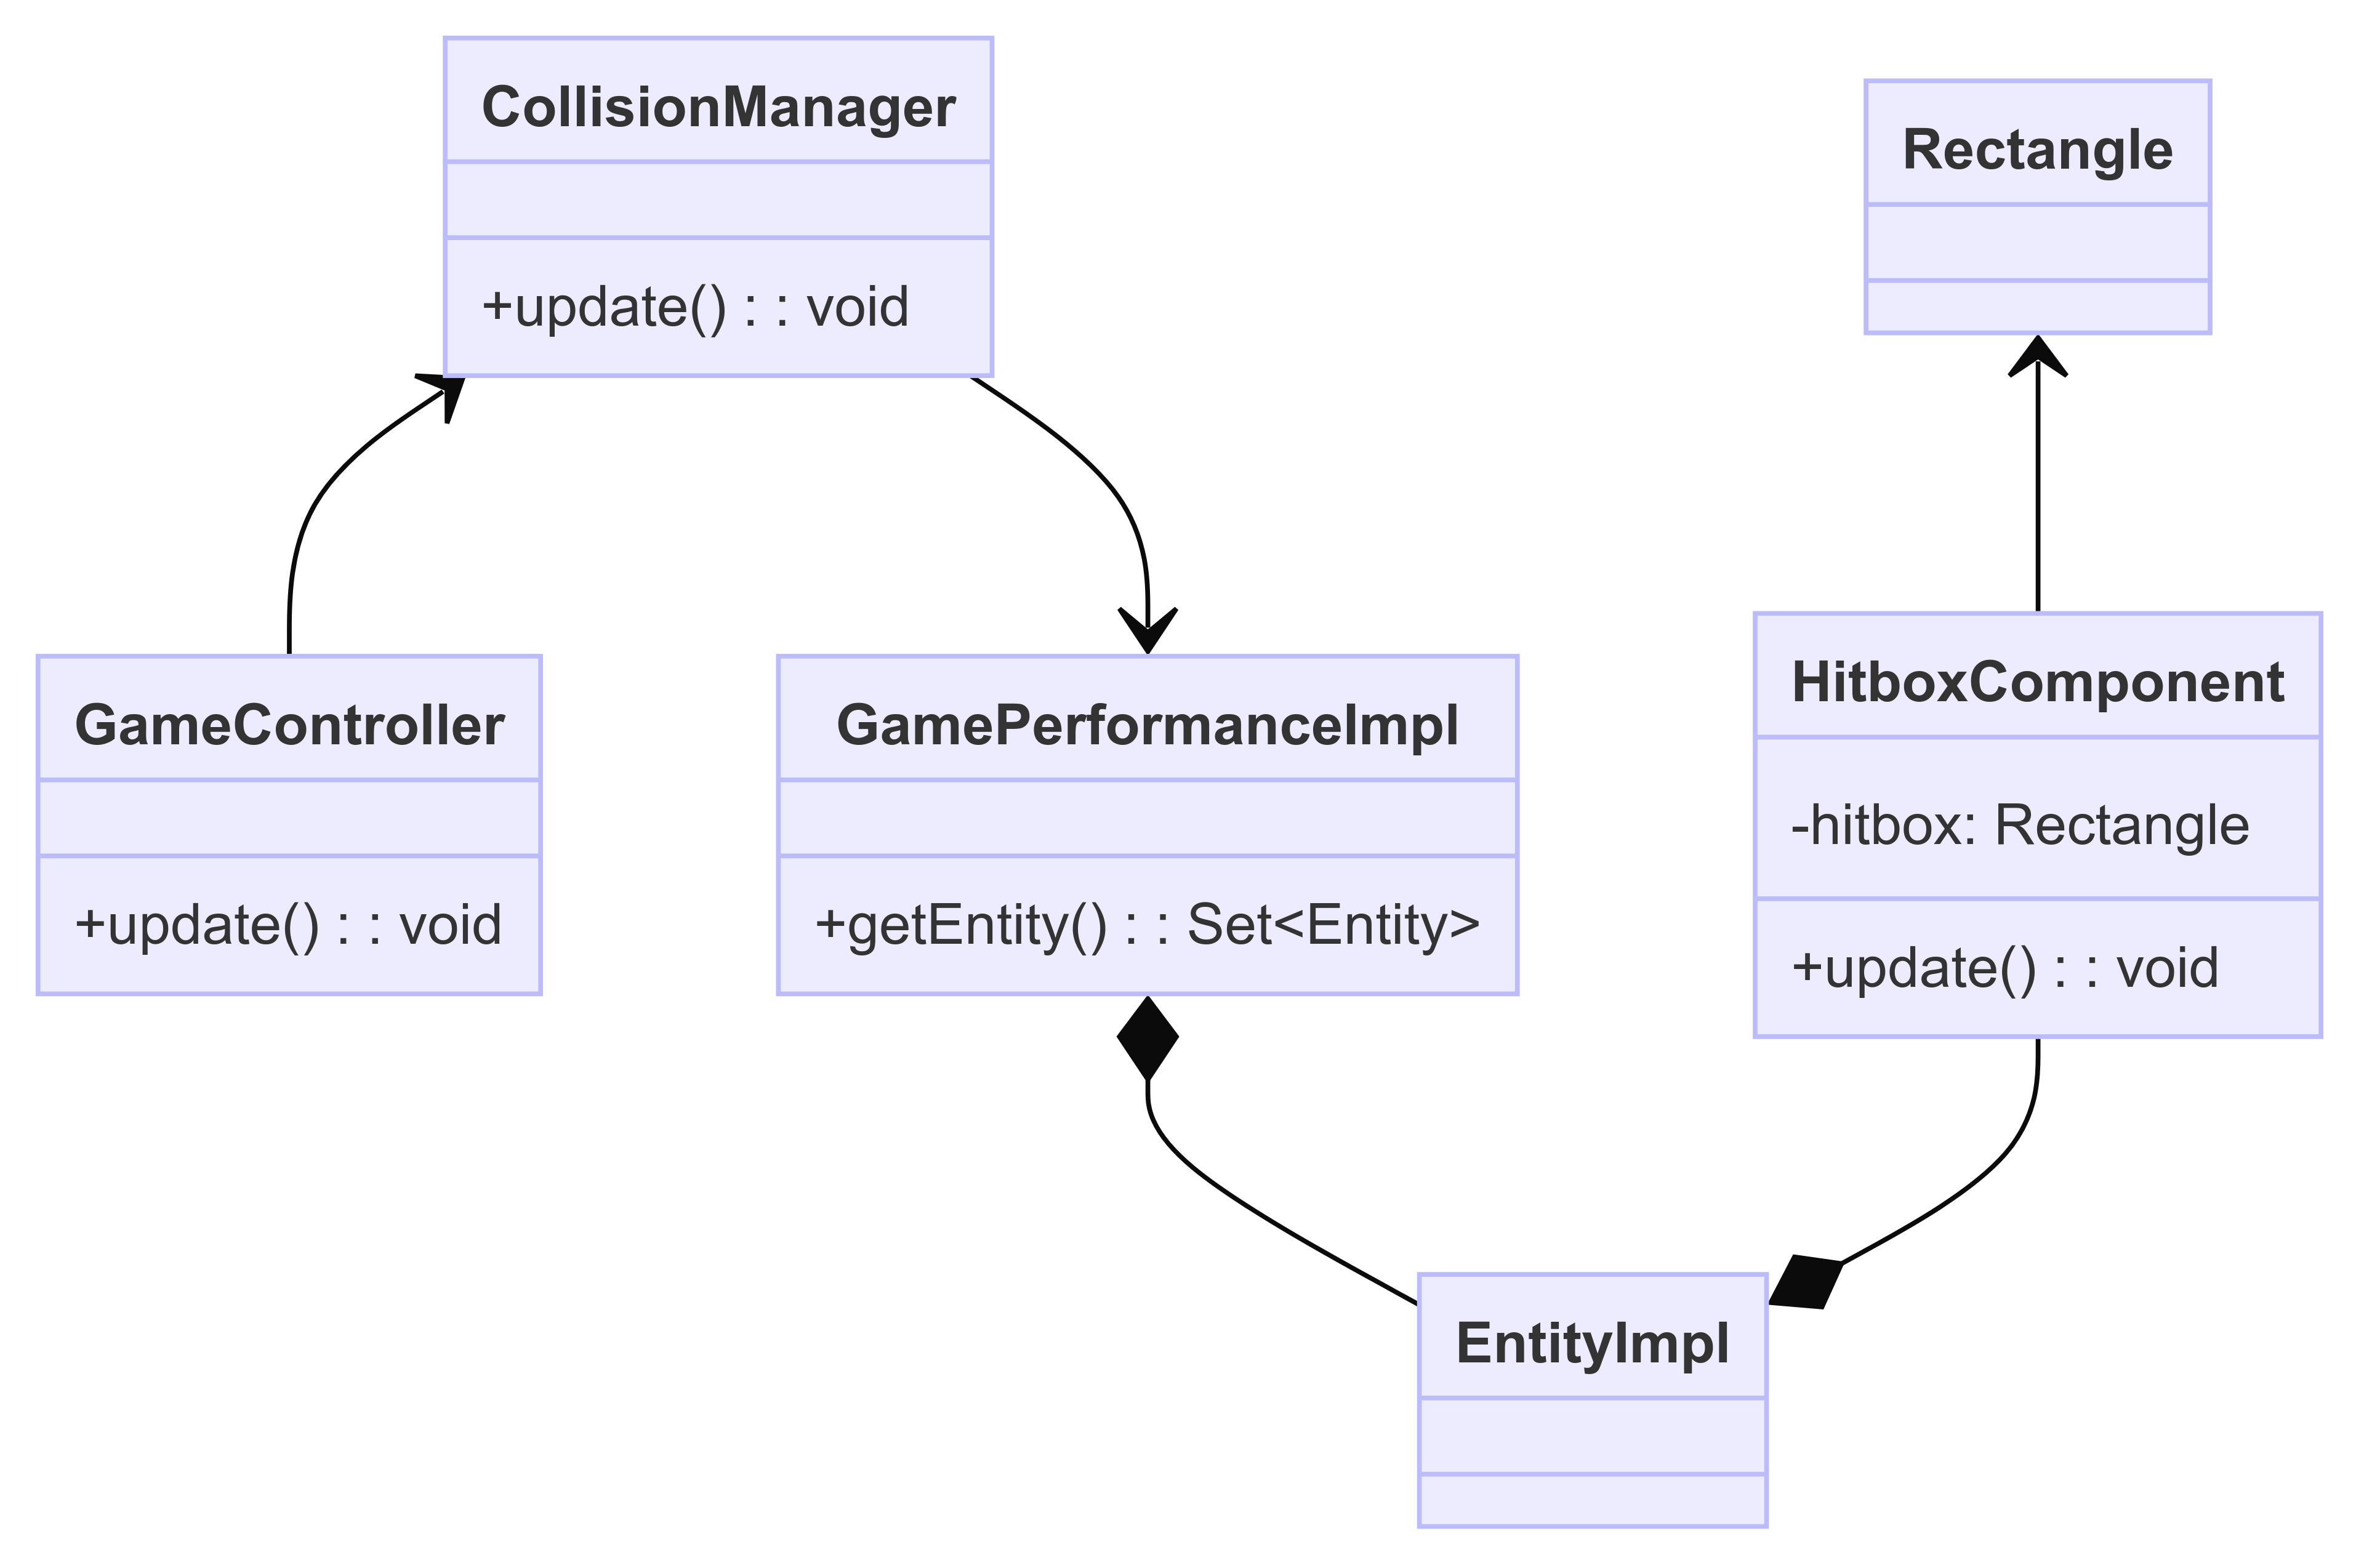
\includegraphics[width=0.9\textwidth]{img/collisions.png}
\caption{Rappresentazione UML della gestione delle collisioni tra entità.}
\end{figure}

\paragraph{Problema:}
Come gestire le collisioni tra le varie entità in modo dinamico, permettendo quindi aggiunte e rimozioni di entità di varie tipologie e cambiamenti di stato.

\paragraph{Soluzione:}
Per poter gestirle ho scelto un pattern Observer che permette di cambiare stato di certe entità observer a seconda di una collisione o no tramite l'observable CollisionManager e se vengono introdotte nuove entità la classe CollisionManager ha in suo possesso già il nuovo insieme. Ciò permette anche la creazione in futuro di altre entità, con caratteristiche nuove, senza dover cambiare la classe CollisionManager, ma bisogna aggiungere le nuove interazioni tra le nuove tipologie di entità e le preesistenti all'interno del metodo update() della classe HitboxComponent. In particolare, in quest'ultima classe lo Strategy pattern sarebbe potuto essere utilizzato nella gestione delle varie casistiche di collisione, permettendo di creare delle ulteriori componenti che gestiscono le collisioni tra certe entità, facilitando anche la gestione, ad esempio, di casi particolari come la collisione tra le entità finestra e Felix.


\subsection{Golesano Giulia}

\subsubsection{Gestione della schermata di gioco}

\begin{figure}[H]
\centering{}
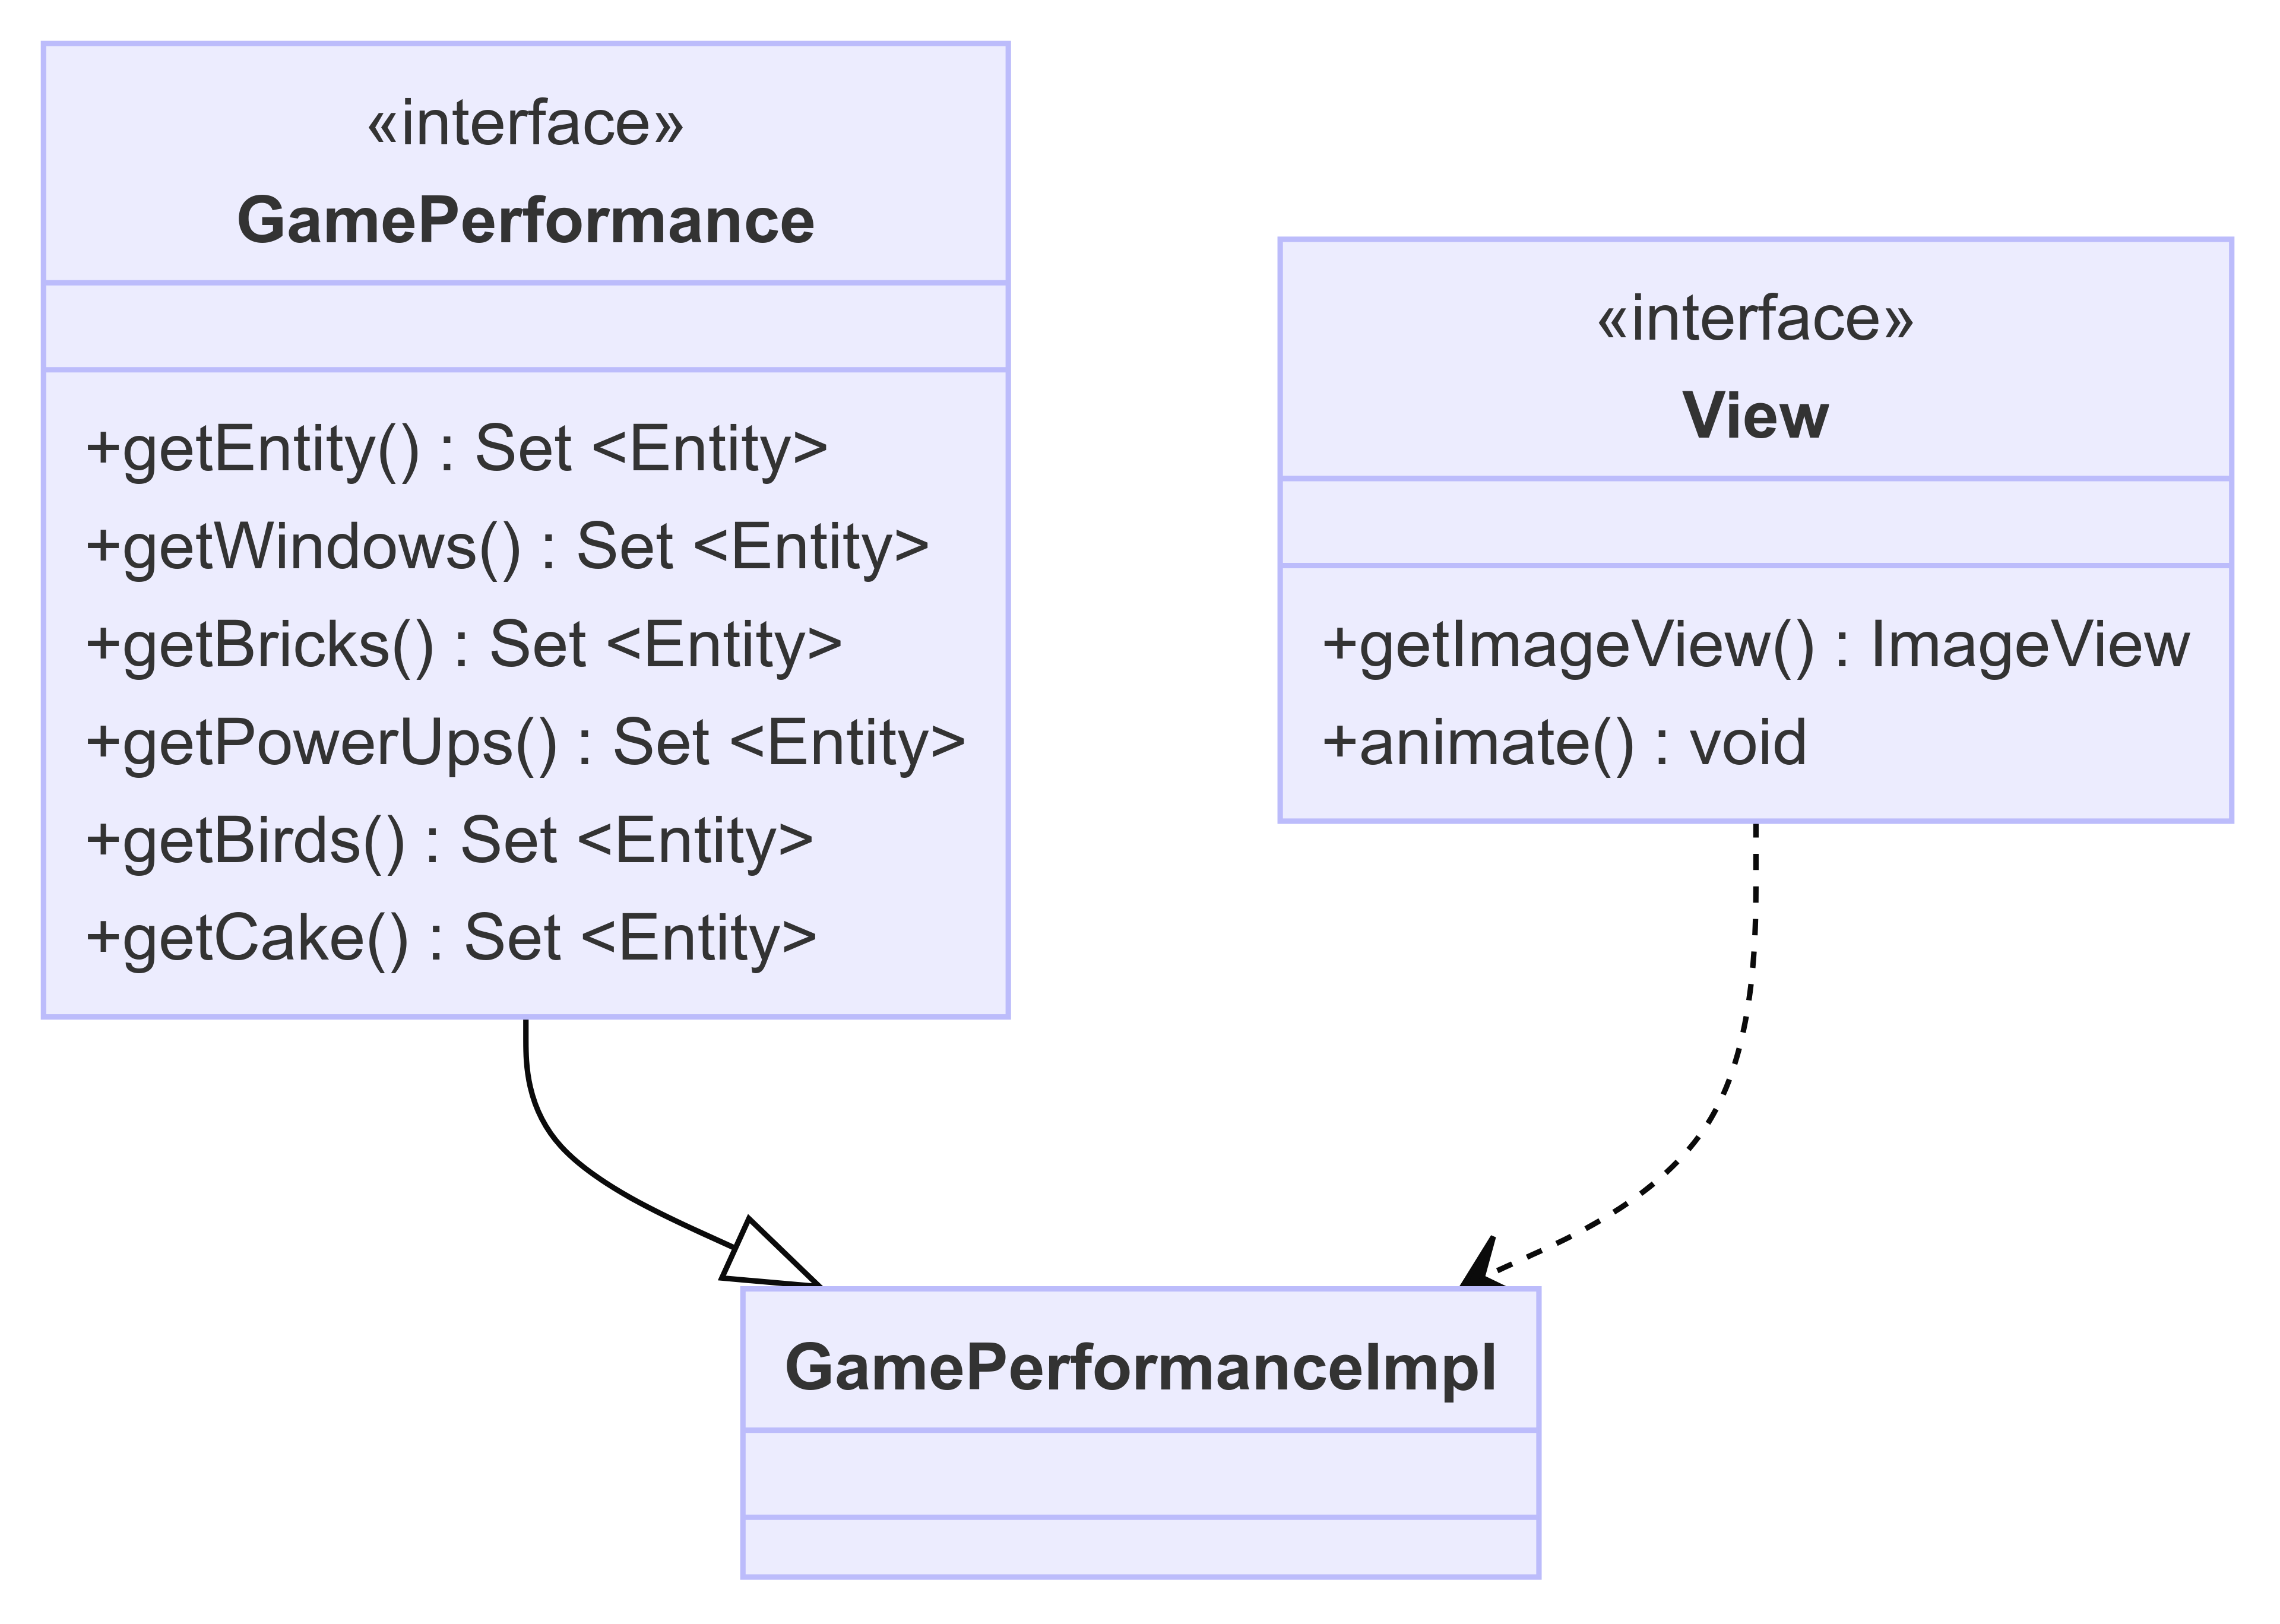
\includegraphics[width=0.4\textwidth]{img/game.png}
\caption{Rappresentazione UML della gestione della schermata di gioco.}
\end{figure}

\paragraph{Problema:}
Gestione della schermata di gioco: inserimento, eliminazione e controllo di ogni entità presente sul campo di gioco, con successiva rappresentazione grafica di esse.
Implementazione di classi View per ogni entità, cosi da realizzare le animazioni e aggiungere gli elementi grafici del gioco.

\paragraph{Soluzione:}
Ho creato un'interfaccia GamePerformance e una implementazione GamePerformanceImpl.
Sono importanti perché fanno un "resoconto" di tutti gli elementi di Model del progetto, cosi da permettere alle classi di View e Controller di accedervi da li.
Ho realizzato un'interfaccia View, che per ogni entità, cerchi l'immagine tra le risorse, realizzi l'animazione o estrapoli il frame desiderato dal png.
Ogni componente del gruppo, successivamente, per realizzare la grafica dei propri elementi, si è appoggiato a tale interfaccia per mantenere un ordine di implementazione simile.

\subsubsection{Gestione degli input }

\begin{figure}[H]
\centering{}
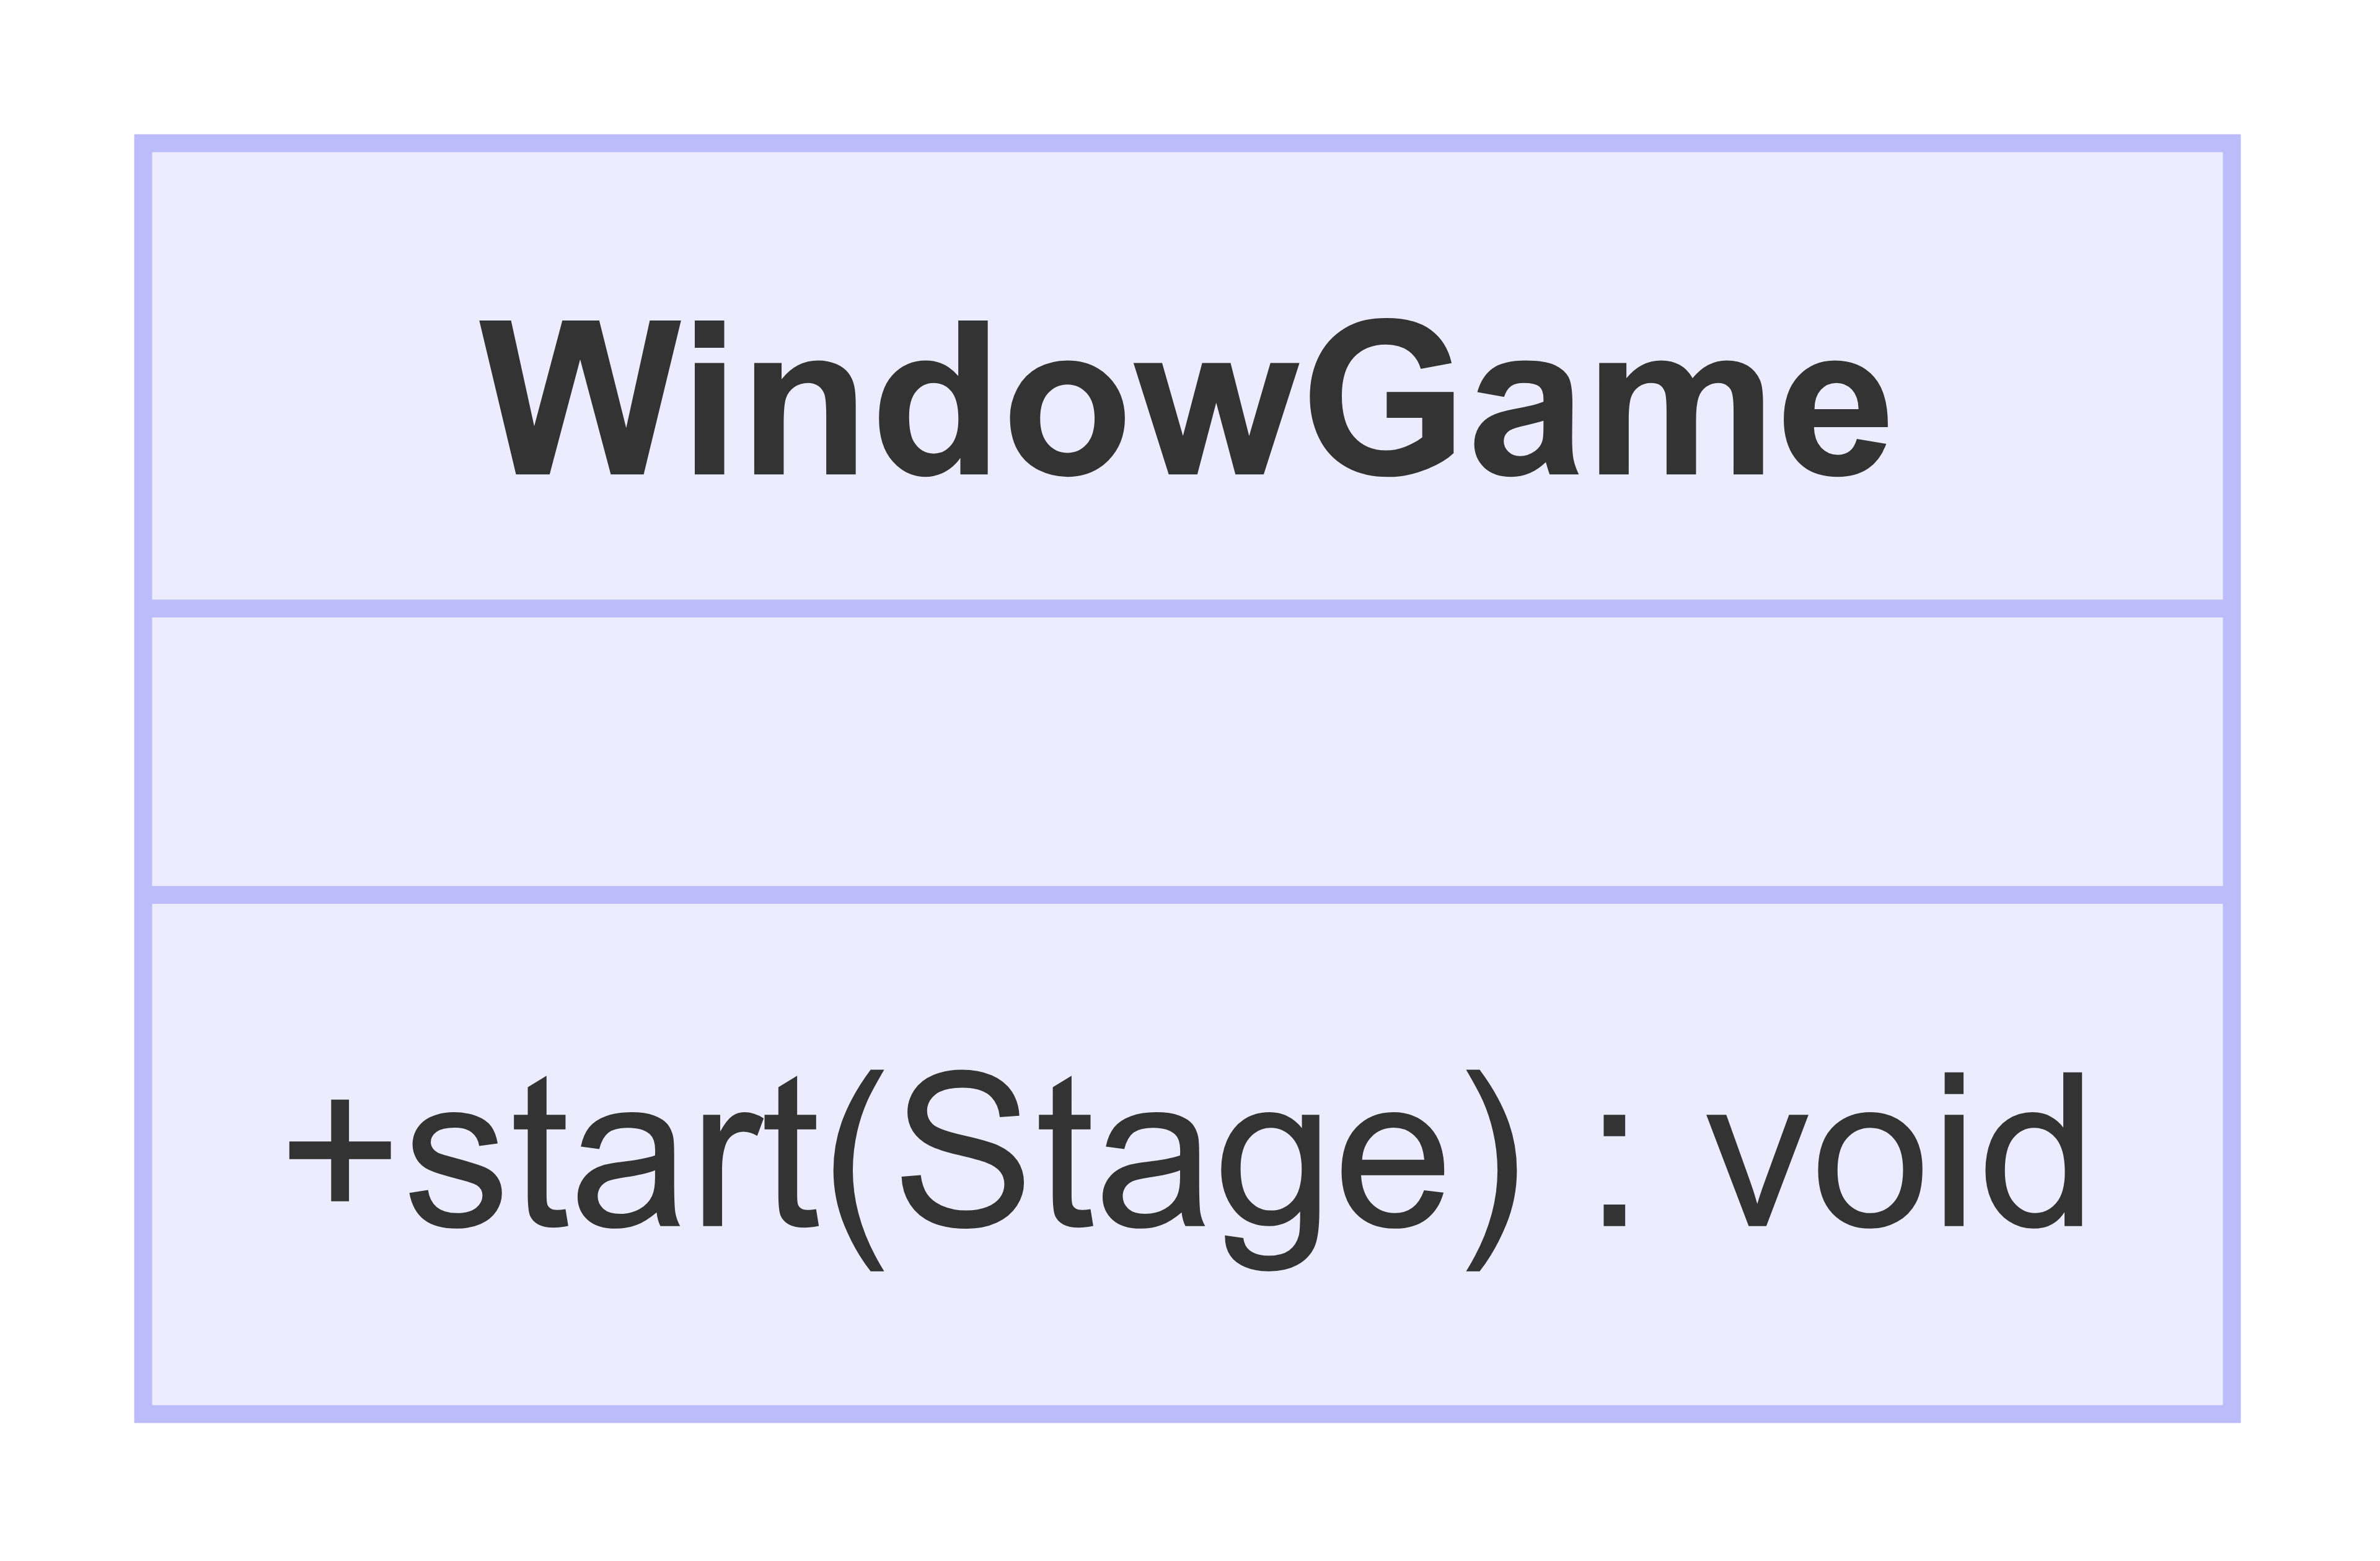
\includegraphics[width=0.4\textwidth]{img/input.png}
\caption{Rappresentazione UML della gestione listener generici di input da tastiera e mouse.}
\end{figure}

\paragraph{Problema:}
Per giocare è necessario far muovere il giocatore sulla schermata di gioco, cliccare sui pulsanti e premere i tasti giusti per aggiustare le finestre.

\paragraph{Soluzione:}
La classe principale che si occupa di tale compito è WindowGame, che contiene la scena principale del gioco, alla quale si appoggiano gli input, grazie ai metodi di Javafx setOnKeyPressed e setOnKeyRealeased.
Tale input, una volta riconosciuto, passa attraverso il controller generico per raggiungere quello desiderato, che compierà l'azione richiesta dallo specifico tasto.

\subsubsection{Creazione delle finestre}

\begin{figure}[H]
\centering{}
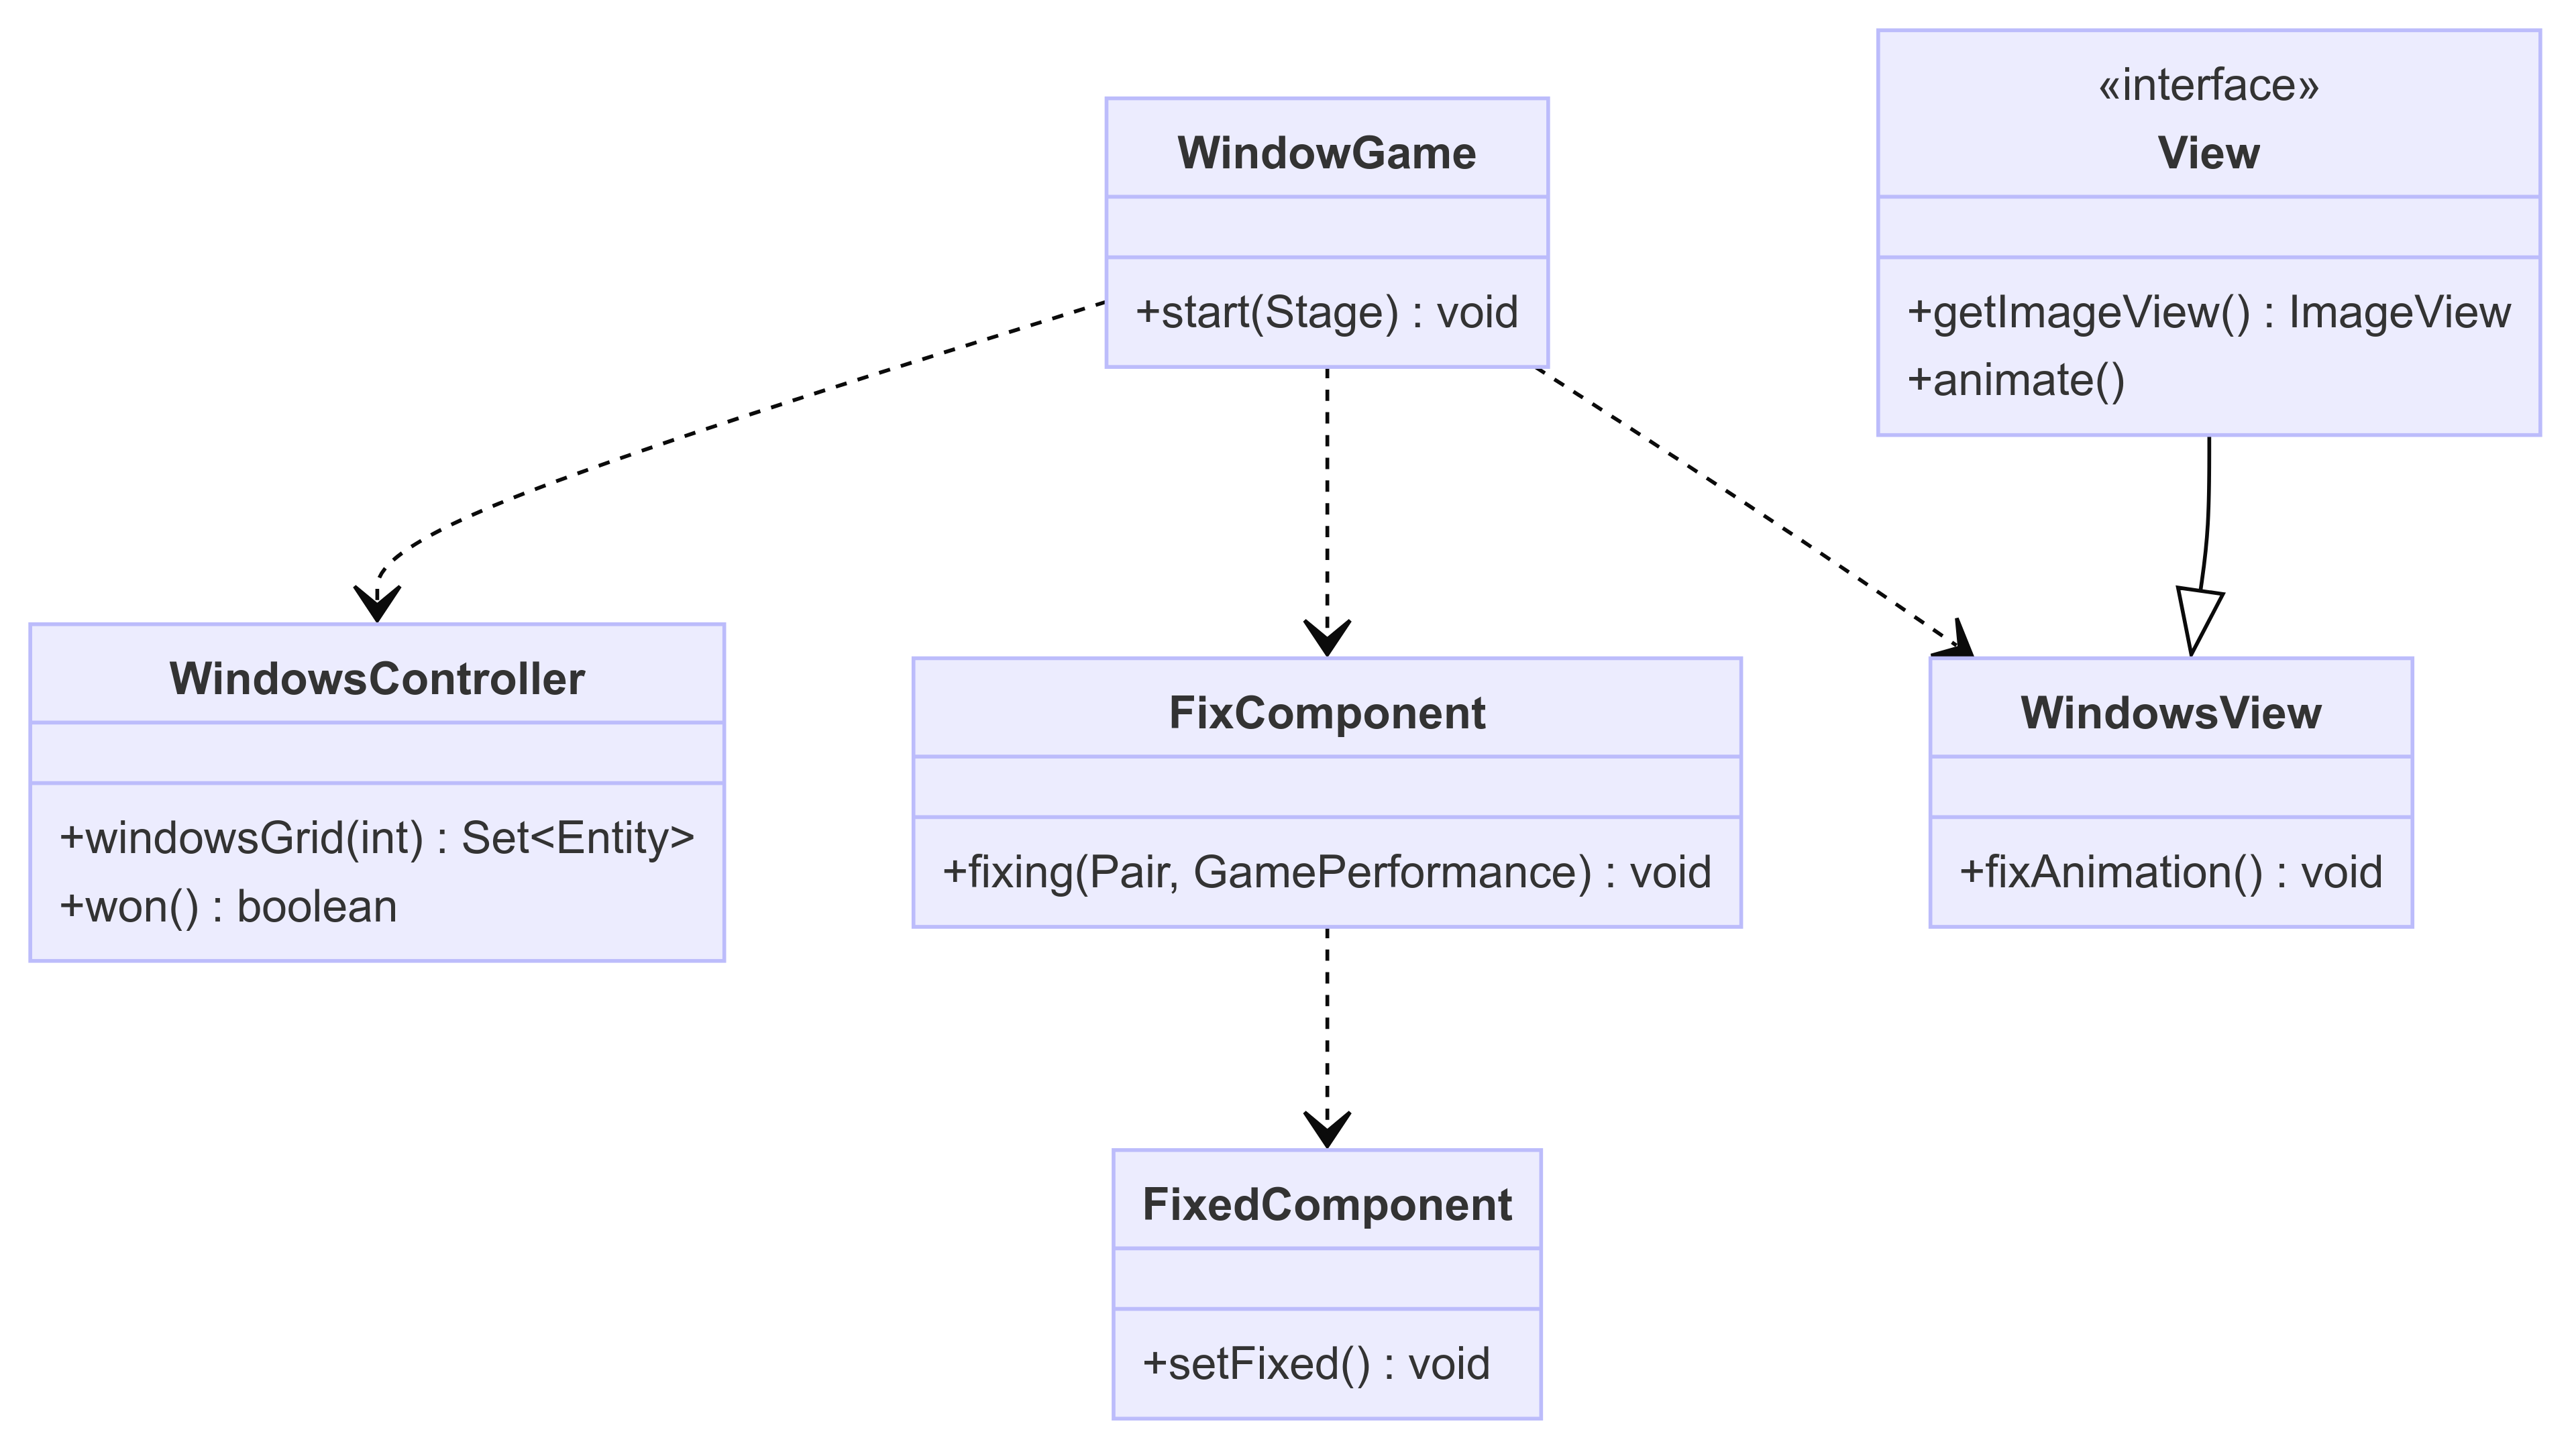
\includegraphics[width=0.4\textwidth]{img/windows.png}
\caption{Rappresentazione UML della gestione delle collisioni.}
\end{figure}

\paragraph{Problema:}
Il campo di gioco si compone principalmente da una griglia di 3x5 finestre, ognuna delle quali è un'entità a se stante, con la caratteristica di essere integra o rotta, a inizio partita.
La condizione di vittoria è avere ogni entità finestra aggiustata.

\paragraph{Soluzione:}

Ho realizzato le classi WindowsController, FixWindowsComponent, FixedWindowsComponent e WindowsView per la gestione di questo problema. 
I component  si occupano di conferire alle entità la capacità di aggiustare finestre e la capacità di essere aggiustate.
FixWindowsComponent, associato all'entità Felix, si occupa di ricercare la finestra che sta entrando in collisione con Felix, e, tramite la sua posizione, impostare il suo campo booleano a True.
FixedWindowsComponent, associato ad ogni finestra in maniera indipendente, si occupa della gestione di questo valore booleano.
La classe principale che si occupa della schermata di gioco, WindowGame, dopo aver controllato il livello, richiama WindowsController, che ha il compito di creare la griglia di finestre e controllare le condizioni di vittoria.
Poi, di nuovo WindowGame, seguendo la griglia appena creata, richiama ogni WindowsView.



\subsection{Rinchiuso Giovanni}

\subsubsection{Gestione del GameEngine}

\begin{figure}[H]
\centering{}
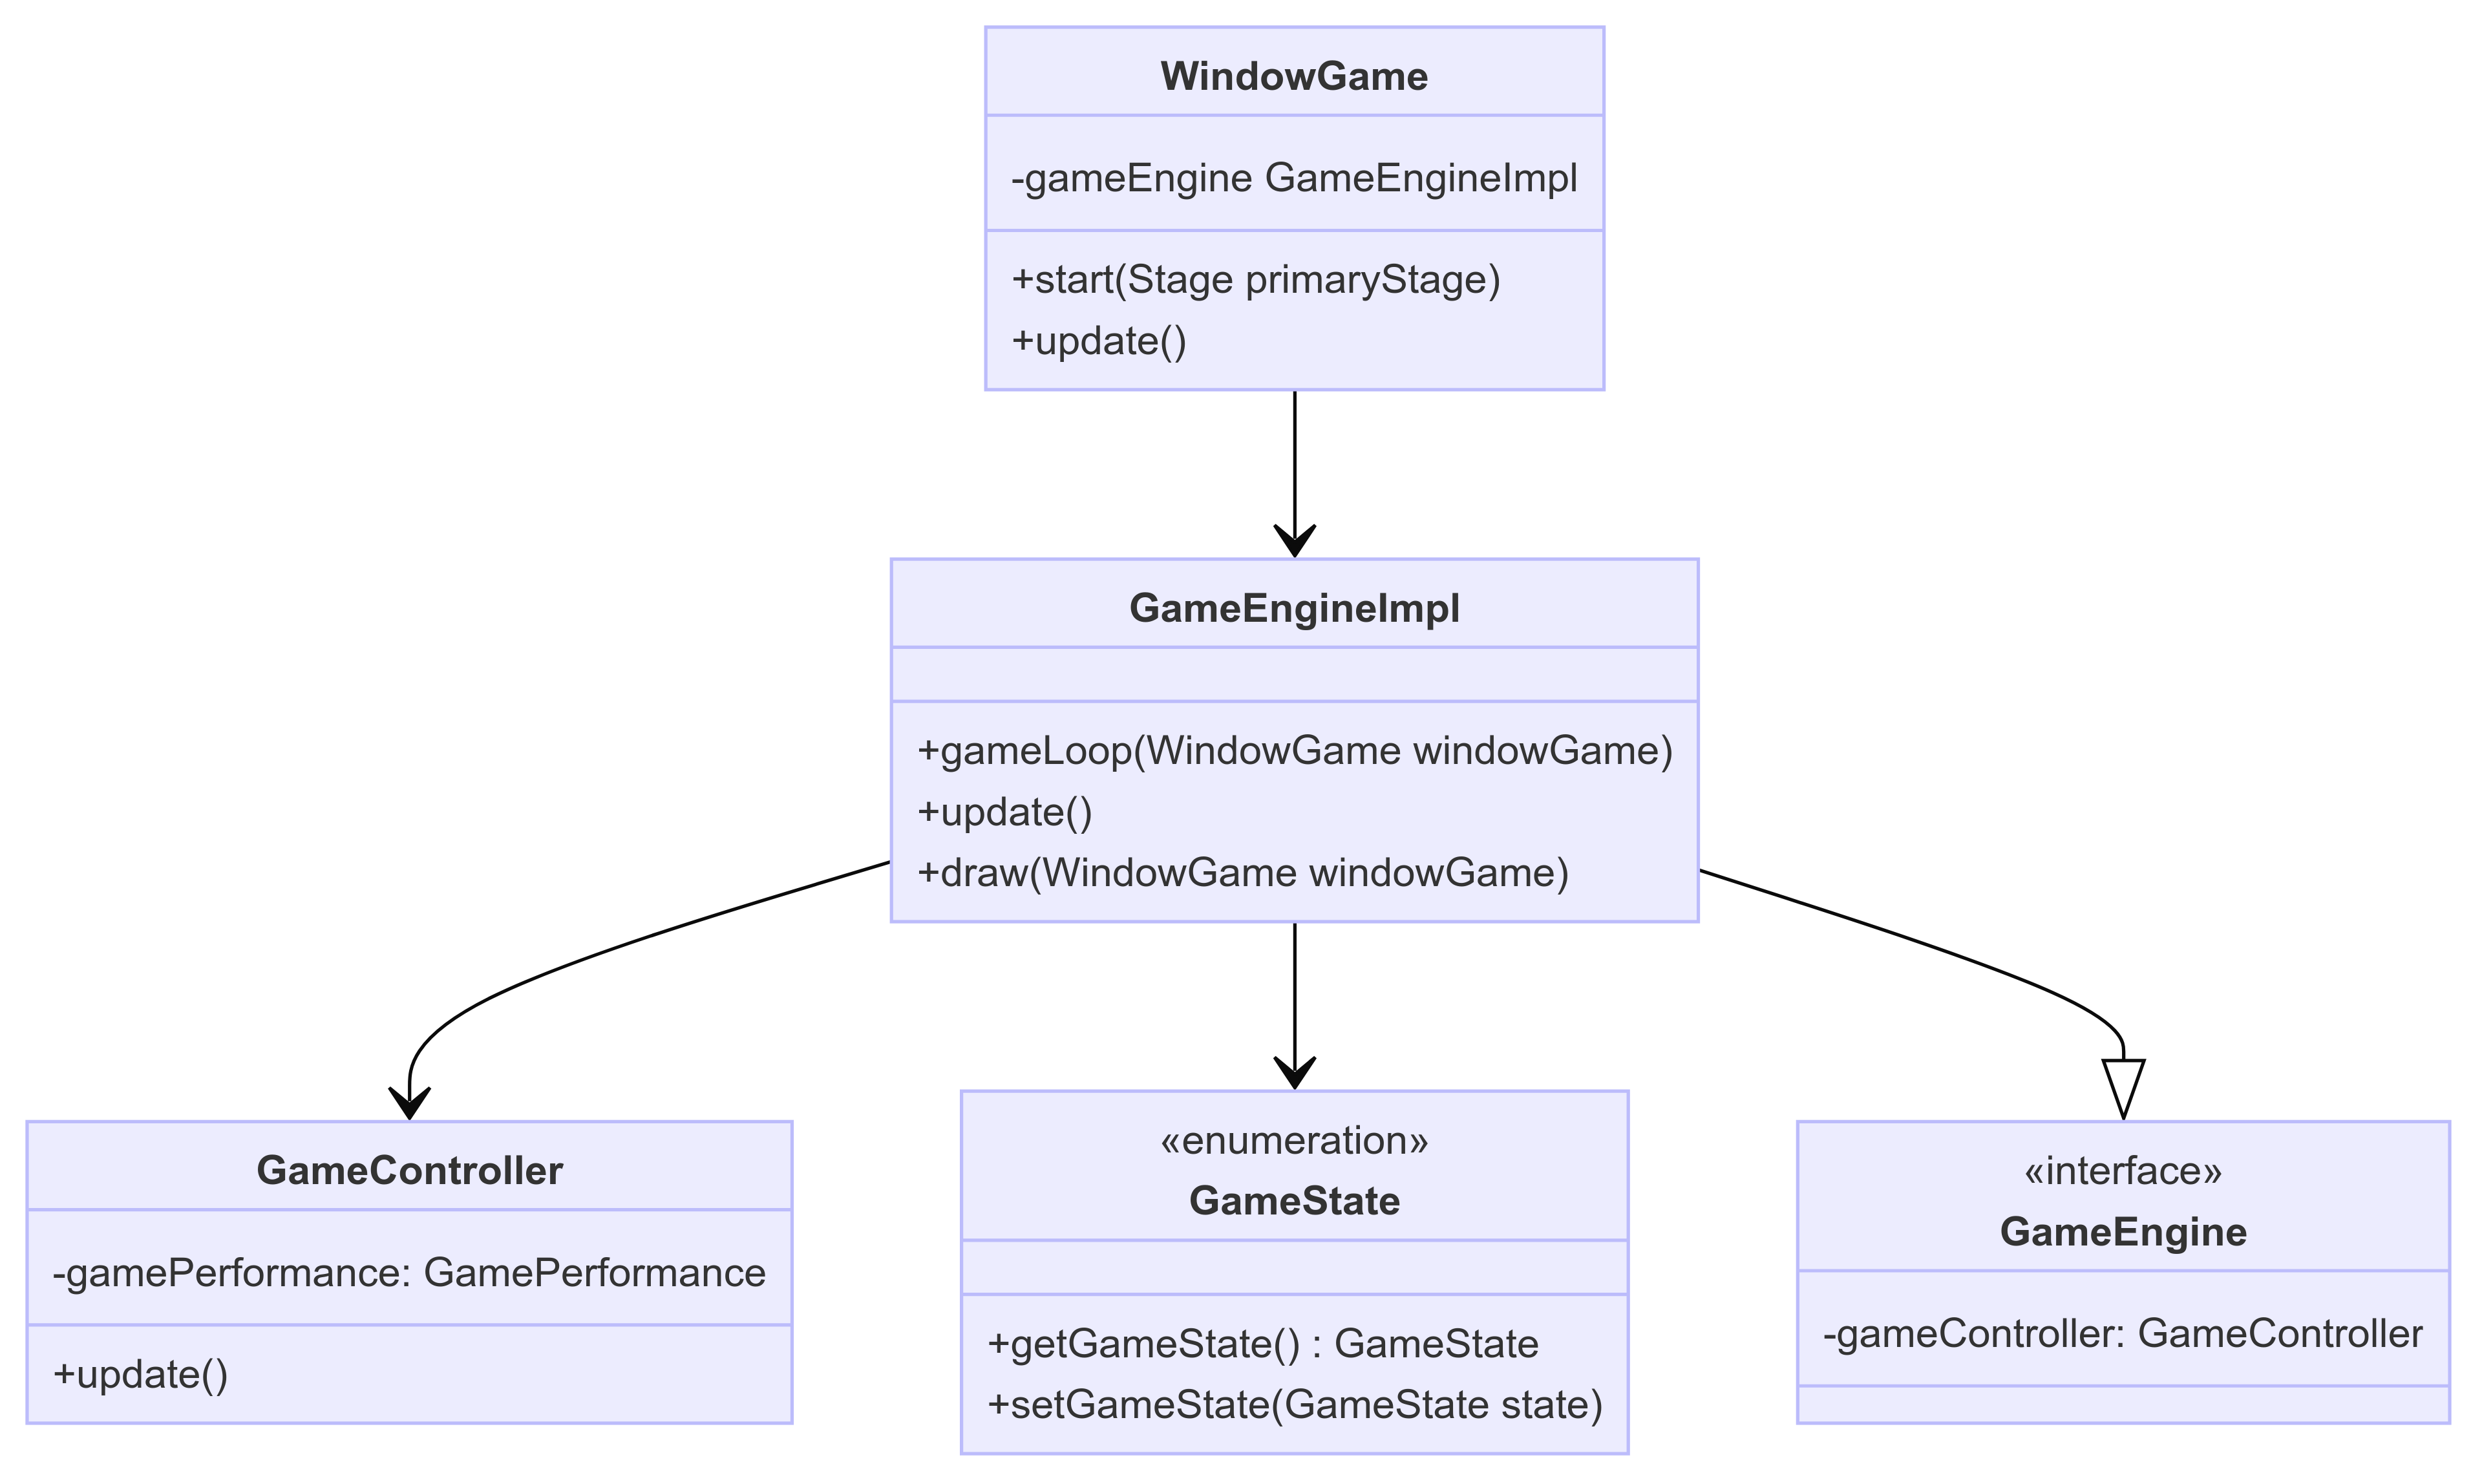
\includegraphics[width=0.4\textwidth]{img/GameEngine.png}
\caption{Rappresentazione UML del game engine.}
\end{figure}

\paragraph{Problema} Il gioco deve essere in grado di permettere un gameplay fluido senza lag, aggiornando ciclicamente la grafica (view) e la logica di gioco (model) in contemporanea.

\paragraph{Soluzione} Ho deciso di scorporare la gestione del game loop dal controller principale (GameController) implementando un’interfaccia GameEngine, al fine di evitare la condivisione di codice sensibile e garantire una maggiore indipendenza, permettendo così di estendere anche in altre classi, in caso di bisogno, il motore del gioco. All'avvio del gioco viene richiamato il metodo start() di WindowGame, che dopo aver disegnato la schermata principale, utilizza la classe AnimationTimer e più in particolare il suo metodo handle(long now), per ciclare ed eseguire il metodo gameLoop() di GameEngine. Tuttavia, durante lo sviluppo, mi sono reso conto che è necessario aggiornare la parte di model e gestione delle varie entità solo nel caso in cui si stia effettivamente giocando; per questa ragione il metodo handle prevede che nel caso in cui ci si trovi nel menù di pausa, venga aggiornata solo la grafica e non venga aggiornata invece la logica di gioco, risparmiando memoria e processi inutili. Invece se il GameState è GAMEOVER o WIN il metodo handle interrompe il suo ciclo e successivamente viene richiamata la grafica corrispondente. 

\subsubsection{Gestione di inizio gioco}

\begin{figure}[H]
\centering{}
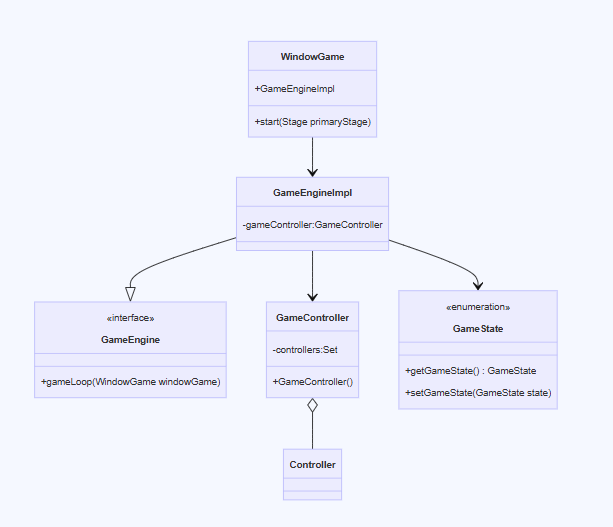
\includegraphics[width=0.4\textwidth]{img/Inizio Gioco.png}
\caption{Rappresentazione UML della logica di inizio gioco.}
\end{figure}

\paragraph{Problema} Avviare una partita in maniera totalmente indipendente ed efficace in qualunque momento e stato dell’applicazione.

\paragraph{Soluzione} Per permettere che una nuova partita possa essere sempre iniziata quando viene premuto il tasto "Start Game" e selezionato il livello, ho implementato il costruttore del GameEngine, che richiama il costruttore del controller principale GameController, che richiama a sua volta i costruttori di tutti gli altri controller, i quali provvedono eventualmente a creare le varie entità del gioco. Il costruttore di GameEngine viene richiamato nel metodo start() del WindowGame, nel quale il gioco entra ogni volta che dalla home, la StartGameView, viene premuto il tasto "Start Game" e selezionato il livello. Ho utilizzato il pattern Strategy, in particolare ho creato un'interfaccia Controller con un metodo update che aggiorna il model. Tutte le altre classi controller come FelixController, RalphController, BrickController, CollisionManager ecc., implementano questa interfaccia, implementando il proprio metodo update. Il GameController ha al suo interno un Set di Controller e delega l'aggiornamento ai vari controller presenti nel Set. 

\subsubsection{Gestione di fine gioco}

\begin{figure}[H]
\centering{}
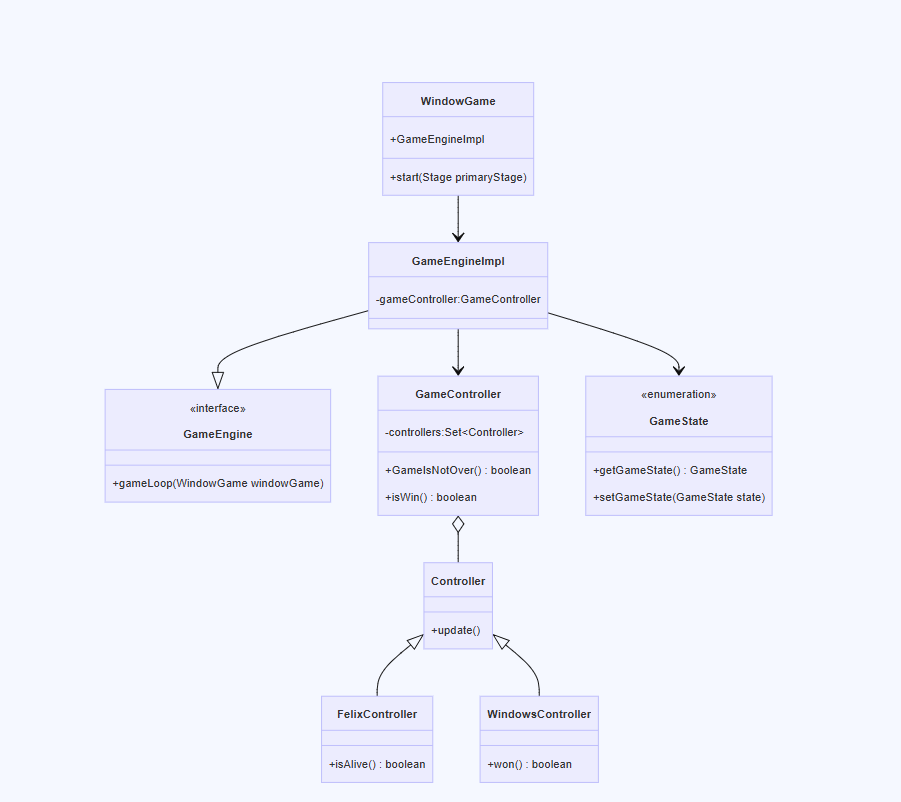
\includegraphics[width=\textwidth]{img/finegioco.png}
\caption{Rappresentazione UML della logica di fine gioco.}
\end{figure}

\paragraph{Problema} Controllare che il giocatore abbia perso o vinto una partita.

\paragraph{Soluzione} Per fare in modo che fosse verificata la condizione di vittoria e sconfitta e fosse aggiornato il Gamestate, effettuo dei controlli all'interno del metodo gameLoop() del gameEngine. Questi controlli vengono quindi eseguiti ogni volta che la funzione handle richiama il metodo gameLoop(). Questi if in particolare controllano tramite metodi implementati nei Controller, che la partita non sia nè vinta nè persa. Nel caso la partita sia vinta, metodo won() del WindowsController, vero se tutte le finestre sono state aggiustate, il GameState viene messo a WIN, mentre se la partita è stata persa, metodo isAlive() del FelixController, che è falso quando Felix viene colpito tre volte da un mattone, il GameState viene messo a GAMEOVER. La funzione handle è implementata in modo per cui se il GameState è GAMEOVER o WIN, smette di ciclare e richiama le opportune view. 

\subsubsection{Gestione dei mattoni}

\begin{figure}[H]
\centering{}
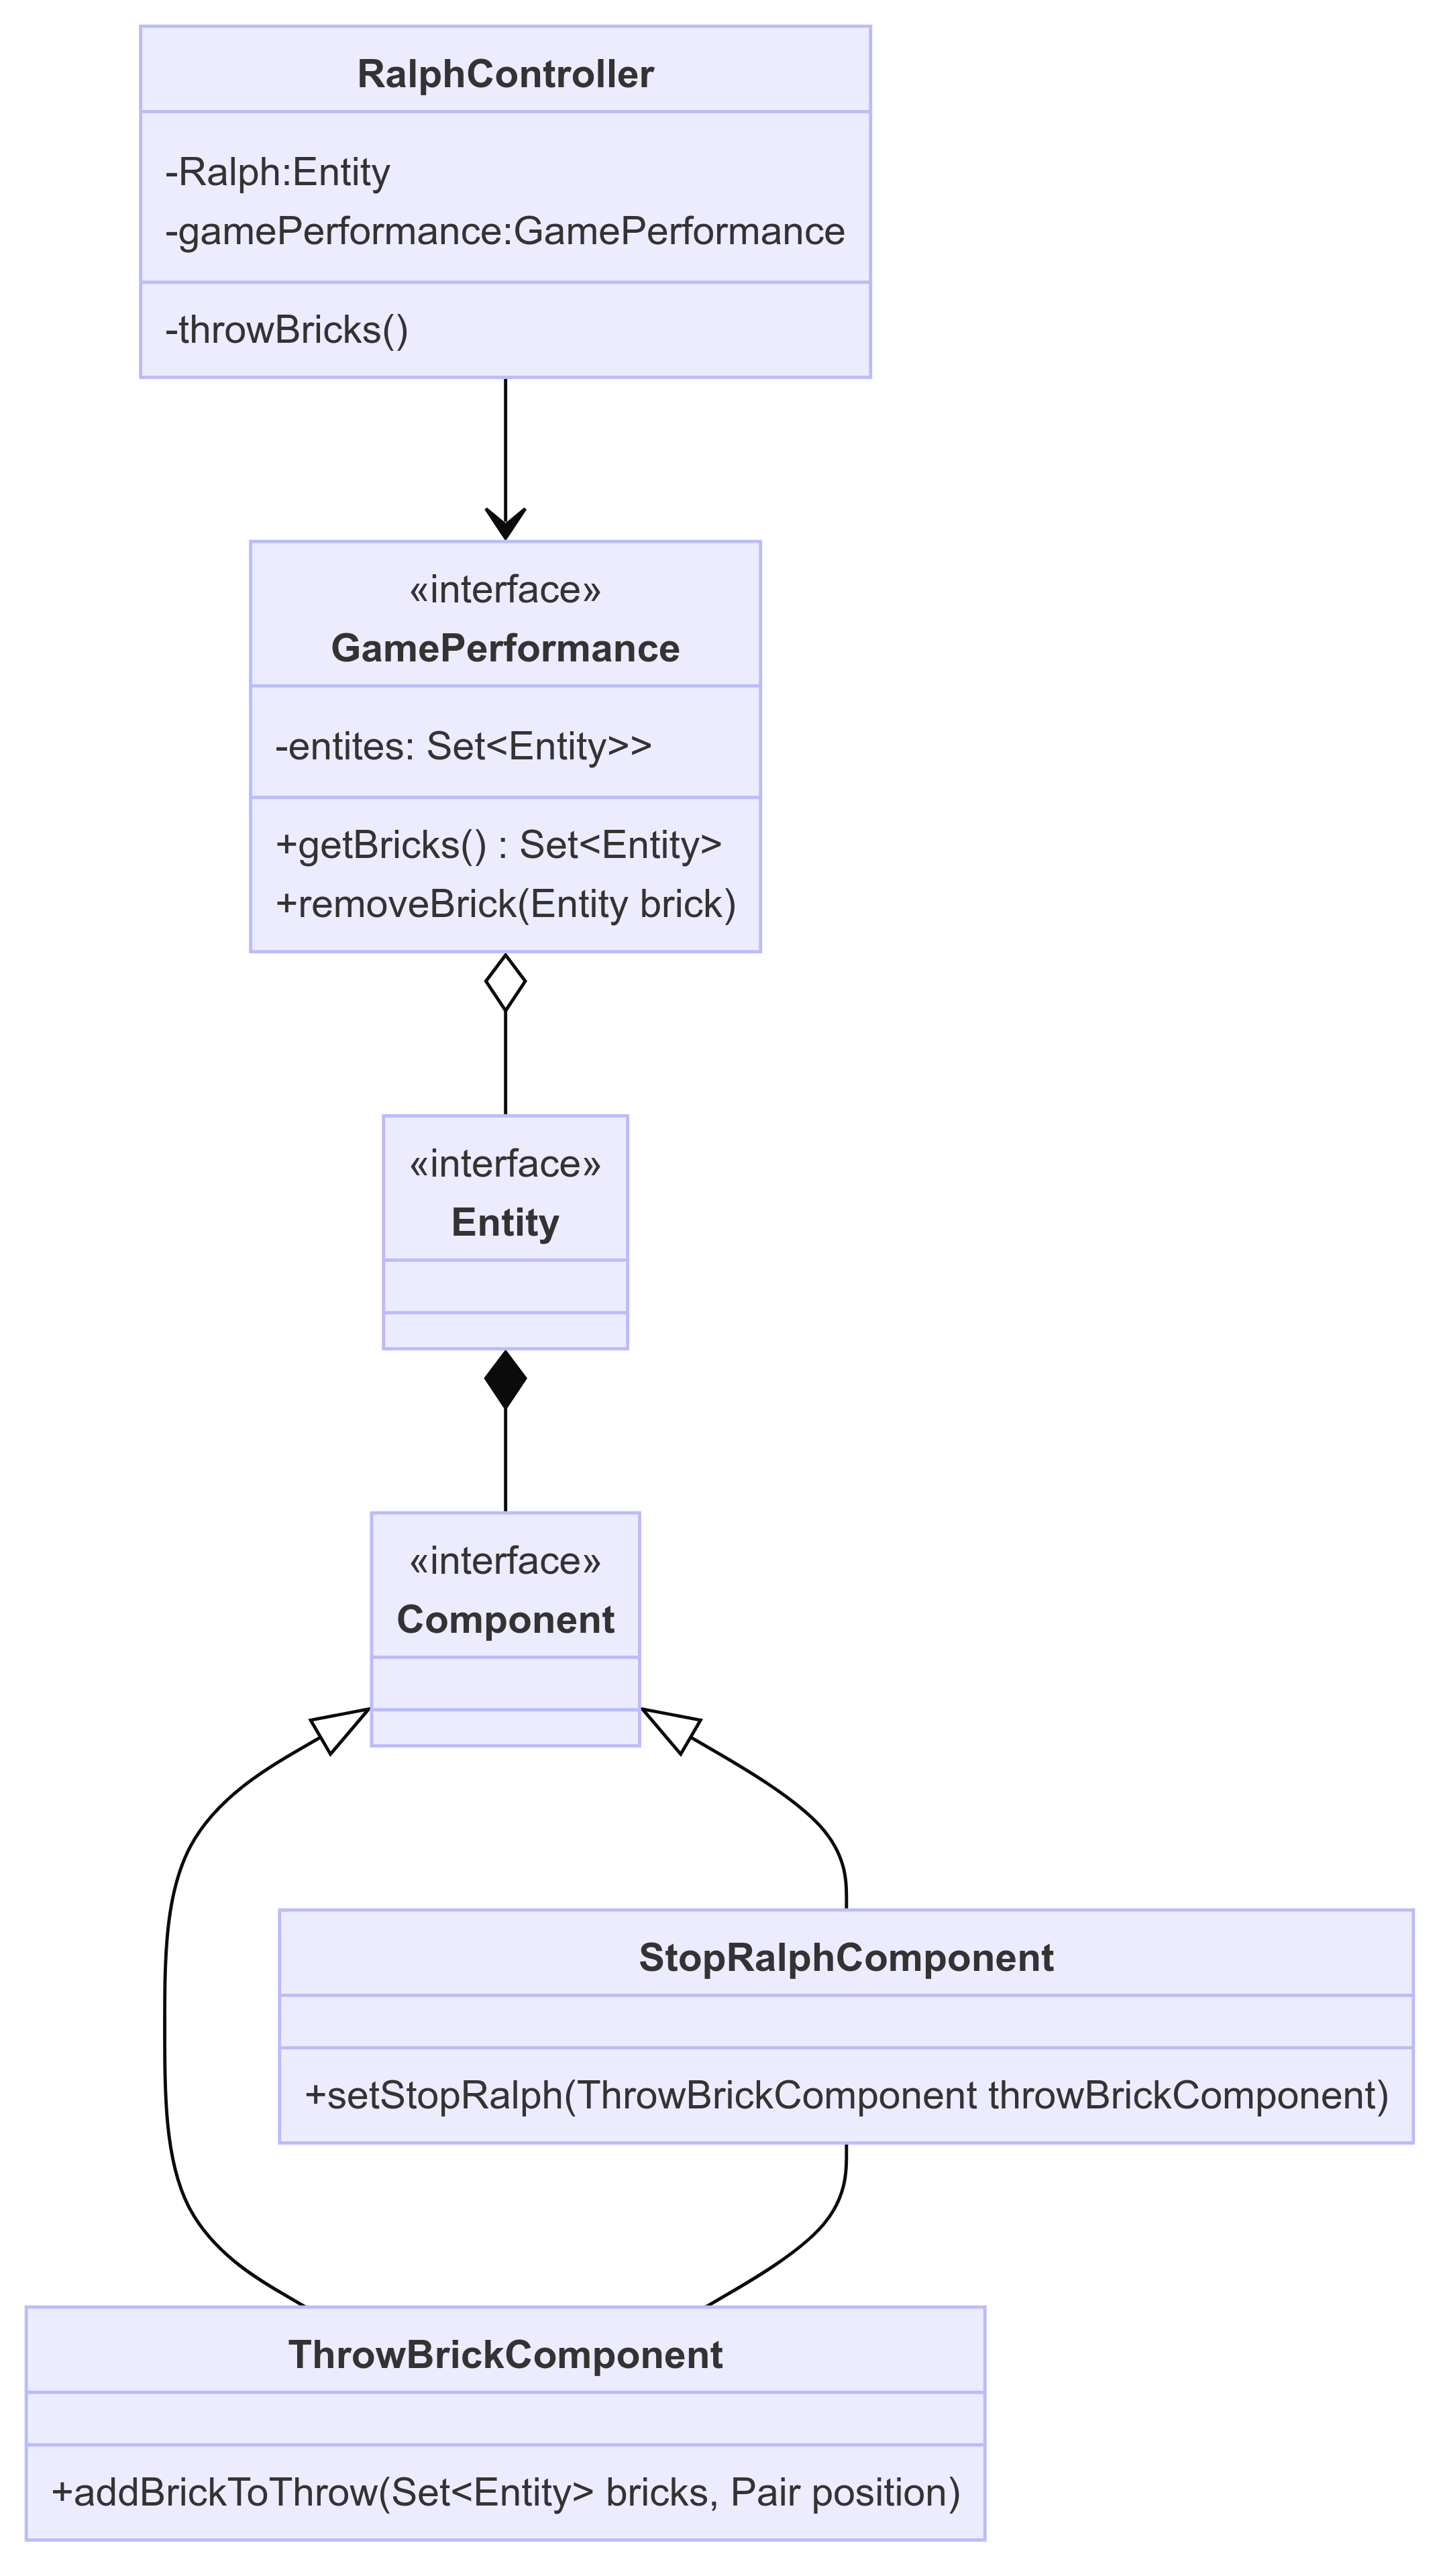
\includegraphics[width=0.4\textwidth]{img/Mattoni.png}
\caption{Rappresentazione UML della logica di spawn dei mattoni e la loro caduta.}
\end{figure}

\paragraph{Problema} Gestione dello spawn dei mattoni durante la partita, farli cadere e rimuoverli una volta che superano i confini della schermata.

\paragraph{Soluzione} Per gestire la generazione delle entità mattoni durante la partita da parte del nemico (Ralph), ho implementato un Component da associare a Ralph, ThrowBrickComponent che estende la classe AbstractComponent. Quando Ralph viene creato nell'EntityFactory, gli viene associato un ThrowBrickComponent, quando viene richiamato il metodo update del GameController(), delega al RalphController il compito di lanciare mattoni. In particolare nel RalphController ci sono due metodi per generare mattoni nelle posizioni della mano sinistra e della mano destra di Ralph ad ogni intervallo di tempo, il quale varia a seconda del livello selezionato. 
Questi metodi utilizzano il metodo addBricks() del ThrowBrickComponent di Ralph per generare questi nuovi mattoni, il quale crea i mattoni (solo se Ralph non è stato bloccato dallo StopRalphComponent) e li aggiunge alla lista di entità presente nel GamePerformance. Sempre nel GamePerformance è presente un metodo getBricks() che restituisce, dell'intera lista di entità solo i mattoni. La caduta dei mattoni viene gestita invece dal BrickController, dal metodo fallBricks(), che fa cadere i mattoni, grazie al metodo move() del MovementComponent, ad una velocità che dipende dal livello selezionato. Il metodo fallBricks(), prima di far cadere i mattoni, chiama il metodo checkBricks(), il quale utilizzando il metodo canMove() del MovementComponent, controlla che i mattoni possano muoversi, se sono arrivati in fondo li rimuove dalla lista di entità presente nel GamePerformance tramite il metodo removeBrick. 

\chapter{Sviluppo}
\section{Testing automatizzato}
Per realizzare i seguenti test è stato utilizzato JUnit 5: 
\begin{itemize}
\item BirdControllerTest, controlla il corretto funzionamento del controller degli uccelli, in particolare la loro creazione e la loro successiva eliminazione.
\item BrickControllerTest, controlla il corretto funzionamento del controller dei mattoni, in particolare la loro caduta e la loro rimozione
\item CakeControllerTest, controlla il corretto funzionamento del controller delle torte, controlla la loro creazione e la loro successiva eliminazione.
\item FelixControllerTest, controlla il corretto funzionamento del controller, in particolare la sua creazione e il suo movimento
\item BirdPositionComponentTest, controlla il corretto funzionamento del BirdPositionComponent.
\item CakePositionComponentTest, controlla il corretto funzionamento del CakePositionComponent.
\item EntityFactoryImplTest, controlla il corretto funzionamento dell'EntityFactoryImpl, in particolare la creazione delle varie entità e la loro corretta associazione ai rispettivi componenti.
\item FixedWindowsComponentTest, controlla il corretto funzionamento del componente delle finestre, controlla che le finestre vengano aggiustate.
\item FixWindowsComponentTest, controlla il corretto funzionamento del componente di Felix, controlla che Felix aggiusti le finestre.
\item ImmortalityComponentTest, controlla il corretto funzionamento del componente di Felix che lo rende immortale per un certo periodo di tempo.
\item LivesComponentTest, controlla il corretto funzionamento del componente delle vite, in particolare controlla che Felix parta con tre vite e che ne perda una in caso di collisione con un mattone.
\item MovementComponentTest, controlla il corretto funzionamento del componente del movimento, controlla che un'entità si muova solo se questo movimento non la porta fuori dai confini della schermata.
\item PointsComponentTest, controlla il corretto funzionamento del componente che calcola i punti, controlla che i punti vengano aggiunti correttamente.
\item StopRalphComponentTest, controlla il corretto funzionamento del componente che blocca Ralph dal lanciare i mattoni. 
\item ThrowBrickComponentTest, controlla il corretto funzionamento del componente che fa lanciare i mattoni a Ralph, controlla che i mattoni vengano aggiunti correttamente. 
\end{itemize}

\section{Note di sviluppo}
\subsubsection{Zanni Nikolai}
\begin{itemize}
    \item Utilizzo di Stream e Lambda expressions:
    \begin{itemize}
        \item \url{https://github.com/giuliagolesano/OOP23-WIR/blob/38de9f235c4600b7bf6ec0aa20f07512825c13df/src/main/java/it/unibo/controller/impl/CakeController.java#L55C4-L59C6}
        \item \url{https://github.com/giuliagolesano/OOP23-WIR/blob/52fc468078493d40b6fe20c39473e2cf277e334d/src/main/java/it/unibo/model/impl/CakePositionComponent.java#L37C4-L53C6}
    \end{itemize}
    \item Utilizzo di Optional:
    \url{https://github.com/giuliagolesano/OOP23-WIR/blob/52fc468078493d40b6fe20c39473e2cf277e334d/src/main/java/it/unibo/view/impl/BaseBirdCakeView.java#L49C2-L56C6}
    \item Utilizzo della libreria JavaFX, usata nella view per realizzare gli sprite animati per Bird e Cake:
    \url{https://github.com/giuliagolesano/OOP23-WIR/blob/52fc468078493d40b6fe20c39473e2cf277e334d/src/main/java/it/unibo/view/impl/BaseBirdCakeView.java#L35C4-L135C2}
\end{itemize}

\subsubsection{Enrico Cornacchia}
\begin{itemize}
    \item Utilizzo di Stream e Lambda expressions piuttosto diffuso in tutto il codice, un esempio che contiene entrambe:
    \url{https://github.com/giuliagolesano/OOP23-WIR/blob/f9343fa68b622f83d4dc34c6fbfbbee61467d4d8/src/main/java/it/unibo/model/impl/HitboxComponent.java#L112C9-L142C20}
    \item Utilizzo di Optional, usati ad esempio per prendere singole componenti di un entità o per certe collisioni:
    \begin{itemize}
        \item \url{https://github.com/giuliagolesano/OOP23-WIR/blob/f9343fa68b622f83d4dc34c6fbfbbee61467d4d8/src/main/java/it/unibo/model/impl/EntityImpl.java#L67}
        \item \url{https://github.com/giuliagolesano/OOP23-WIR/blob/f9343fa68b622f83d4dc34c6fbfbbee61467d4d8/src/main/java/it/unibo/model/impl/HitboxComponent.java#L156C5-L165C6}
    \end{itemize}
    \item Utilizzo della libreria JavaFX, usata nella view per realizzare gli sprite animati per Felix e Ralph, ad esempio:
    \begin{itemize}
        \item \url{https://github.com/giuliagolesano/OOP23-WIR/blob/f9343fa68b622f83d4dc34c6fbfbbee61467d4d8/src/main/java/it/unibo/view/impl/FelixView.java#L58C5-L69C6}
        \item \url{https://github.com/giuliagolesano/OOP23-WIR/blob/f9343fa68b622f83d4dc34c6fbfbbee61467d4d8/src/main/java/it/unibo/view/impl/RalphView.java#L58C5-L73C6}
    \end{itemize}
    \item Progetto Donkey Kong, \url{https://github.com/MattiaSemproli/OOP22-DonkeyKong}, e Game as a lab \url{https://github.com/pslab-unibo/oop-game-prog-patterns-2022} usati come spunto per la realizzazione rispettivamente di entità e collisioni
    \item La classe Pair utilizzata in questo progetto è quella fornita dal professore Mirko Viroli durante il corso
    \item Sprite sheet preso da \url{https://www.spriters-resource.com/pc_computer/fixitfelixjr/}
\end{itemize}

\subsubsection{Golesano Giulia}
\begin{itemize}
    \item Utilizzo di Optional:
        \begin{itemize}
        \item  \url{https://github.com/giuliagolesano/OOP23-WIR/blob/8a691b615a5751d7b0182df54ada557bb310edd6/src/main/java/it/unibo/view/impl/WindowGame.java#L190}
        \end{itemize}
    \item Utilizzo di Stream e Lambda expressions, presenti in più implementazioni, ne riporto un esempio comune:
        \begin{itemize}
        \item  \url{https://github.com/giuliagolesano/OOP23-WIR/blob/8a691b615a5751d7b0182df54ada557bb310edd6/src/main/java/it/unibo/view/impl/WindowGame.java#L285-L300}
        \end{itemize}
    \item Utilizzo della libreria JavaFx per realizzare l'animazione di una finestra che viene aggiustata da Felix:
    \begin{itemize}
    \item \url{https://github.com/giuliagolesano/OOP23-WIR/blob/8a691b615a5751d7b0182df54ada557bb310edd6/src/main/java/it/unibo/view/impl/WindowsView.java#L49-L69}
    \end{itemize}
\end{itemize}
    

\subsubsection{Rinchiuso Giovanni}
\begin{itemize}
\item Utilizzo di Stream e Lambda expressions, presenti in varie parti del codice, ecco un esempio: 
\url {https://github.com/giuliagolesano/OOP23-WIR/blob/main/src/main/java/it/unibo/view/impl/WindowGame.java#L396C13-L400C1}
\end{itemize}

\chapter{Commenti Finali}
\section{Autovalutazione e lavori futuri}

\subsubsection{Zanni Nikolai}
Inizialmente avevo preso alla leggera questo progetto di gruppo, pensando sarebbe stato molto più semplice. Andando avanti, però, mi sono ricreduto e ho notato una mia personale mancanza di approfondimento sulla materia in questione. Man mano che progredivo con il progetto, ho dovuto anche riguardare i vari laboratori e la teoria per poter proseguire.
Lavorare in gruppo ha dato una mano fondamentale, perché in questo modo abbiamo avuto la possibilità di aiutarci tra di noi e di confrontarci. La collaborazione con i miei compagni è stata cruciale per superare le difficoltà e per arricchire la mia comprensione dei concetti più complessi.
In particolare, la parte di View mi è risultata meno impegnativa rispetto alle altre mie parti di codice, dove dovevo capire come fare funzionare model e controller assieme. L'implementazione della View, grazie alla chiarezza delle librerie e delle strutture di JavaFX, è stata più intuitiva e mi ha permesso di visualizzare rapidamente i risultati del mio lavoro. Tuttavia, la sfida è stata integrare le View con il resto dell'architettura MVC, garantendo una comunicazione efficace tra model e controller.
Alla fine di questo progetto, posso dire di aver acquisito una comprensione molto più solida delle tecnologie e dei principi di design utilizzati. Inoltre, il lavoro di squadra mi ha insegnato l'importanza della comunicazione e della collaborazione efficace. Questo progetto è stato una preziosa opportunità di crescita personale e professionale, che mi ha permesso di sviluppare non solo le mie competenze tecniche, ma anche le mie abilità di lavoro in team e di gestione del tempo.

\subsubsection{Cornacchia Enrico}
Questo progetto mi ha insegnato l'importanza della progettazione di software. In particoalre, essendomi occupato per la maggior parte di model e parte del controller, essere partito con un idea precisa di cosa voler fare, mi è stato di grande aiuto, nel realizzare codice funzionante e che non si rompesse alla prima modifica da apportare. Tuttavia, consultando all'inizio un "catalogo" ben realizzato dei pattern di design \href{https://refactoring.guru/design-patterns}{Refactoring Guru}, avevo in mente molteplici idee per realizzare la stessa cosa e alla fine ho sempre scelto l'opzione più semplice, che spesso (come nel caso della gestione delle collisioni) non risulta ottimale. In ogni caso, una volta messo mano al codice non ho riscontrato particolari difficoltà, anzi, sono riuscito a comprendere ancora meglio l'utilità degli stream, che si sono rivelati utilissimi per compattare il codice e, allo stesso tempo, renderlo anche più comprensibile. Effettivamente sono stato impegnato anche in altre parti di codice per aiutare il mio team a risolvere il più velocemente possibile, specialmente a causa di svariati problemi collegati all'utilizzo, nella parte di view, di JavaFX. Sulla risoluzione di bug ci abbiamo lavorato tutti, dividendoci le parti in modo da ottimizzare il tempo al massimo. Considerando il tutto, alla fine di questo progetto posso dirmi relativamente soddisfatto del risultato ottenuto, ma c'è sicuramente margine di miglioramento.

\subsubsection{Golesano Giulia}
Quando ho iniziato a lavorare al progetto mi sentivo molto spaesata e incapace, rispetto ad una reale applicazione di ciò che avevo studiato.
Man mano che i mesi andavano avanti, la possibilità di lavorarci con calma, durante le lezioni, senza la fretta della sessione di esami, mi ha reso sempre più consapevole di come le cose funzionassero e come potevo realizzare le mie idee.
Ho iniziato ad apprezzare e utilizzare con più facilità elementi come gli Stream e le Lambda, essenziali per realizzare in maniera veloce e compatta controlli o modifiche su flussi di dati.
Mi sono presa del tempo per imparare ad utilizzare JavaFX, tramite libri, guide e articoli, e sicuramente, nonostante la difficoltà, sento di aver imparato diverse cose.
Sento inoltre che mi è servito tanto il lavoro di gruppo con i miei compagni, perché ho appreso elasticità rispetto alle velocità e tecniche di lavoro degli altri.
Ci siamo aiutati durante tutto il percorso e, in special modo, nelle ultime settimane, utilizzando i propri punti di forza o conoscenze per aiutare i punti deboli o mancanze del compagno.
Le ore di lavoro sono state tante, diverse anche solo di lettura di articoli e siti web che chiarissero alcune implementazioni, prima di provare ogni cosa appresa sul nostro progetto.
In conclusione, penso che tutto il gruppo abbia fatto un discreto lavoro.

\subsubsection{Rinchiuso Giovanni}
Inizialmente avevo molti timori riguardo a questo progetto, in quanto essendo uno studente al terzo anno, avevo bisogno di superare questo esame per potermi laureare. Inoltre tutti i miei compagni di corso mi hanno sempre parlato di questo progetto come il più stimolante ma anche come il più impegnativo che avessero affrontato. Questa cosa mi spaventava molto, perché credevo di non essere in grado di portarlo a termine, però mi ha anche aiutato ad affrontare questo progetto con il dovuto impegno. E' stato molto stimolante vedere che il nostro gioco diventava sempre più simile a come l'avevamo immaginato. Il gruppo ha lavorato molto bene, è stato gratificante poter contare sull'aiuto degli altri ed essere io stesso utile a loro. Penso che ci siano margini di miglioramento sia per la nostra applicazione, sia per il mio metodo di programmazione, ma penso di essere sulla strada giusta e che il lavoro svolto sia buono. 

\section{Difficoltà incontrate e commenti per i docenti}
\begin{itemize}
    \item Questo progetto è un modo perfetto per imparare il design per software, tuttavia durante le lezioni non mi è sembrato attribuito abbastanza importanza. In laboratorio poi bisognerebbe realizzare più esercizi su tale argomento, un buon esempio è l'esercizio 44-45 rich design del laboratorio 4.
\end{itemize}
\appendix
\chapter{Guida Utente}
L'obiettivo del gioco è aggiustare tutte le finestre, schivando i mattoni lanciati da Ralph e cercando di raggiungere tutti i power ups disponibili.
I comandi di gioco sono:
\begin{itemize}
 \item A: Movimento verso sinistra.
 \item W: Movimento verso l'alto.
 \item S: Movimento verso il basso.
 \item D: Movimento verso destra.
 \item Z: Se premuto per 1.5 secondi aggiusta la finestra in cui si trova Felix.
\end{itemize}
I power ups sono:
\begin{itemize}
 \item Cake: rende immortale Felix per 10 secondi
 \item Bird: Ralph non lancia più mattoni per 10 secondi
\end{itemize}
\chapter{Esecitazioni di laboratorio} 

\section{enrico.cornacchia@studio.unibo.it}

\begin{itemize}
 \item Laboratorio 06: \url{https://virtuale.unibo.it/mod/forum/discuss.php?d=146511#p208416}
 \item Laboratorio 07: \url{https://virtuale.unibo.it/mod/forum/discuss.php?d=147598#p209350}
 \item Laboratorio 08: \url{https://virtuale.unibo.it/mod/forum/discuss.php?d=148025#p210126}
 \item Laboratorio 09: \url{https://virtuale.unibo.it/mod/forum/discuss.php?d=149231#p211607}
 \item Laboratorio 10: \url{https://virtuale.unibo.it/mod/forum/discuss.php?d=150252#p212636}
\end{itemize}

\end{document}